\section{Modulation}
\textbf{HAREC a.\ref{HAREC.a.1.8}\label{myHAREC.a.1.8}}
\label{modulation}
\index{modulation}

\subsection{Allmänt}

\emph{Modulera} (lat. \emph{modulari}, rytmiskt avmäta) är att med hjälp av en
oftast högfrekvent elektrisk signal (bärvågen) överföra informationen i en
lågfrekvent signal. På så sätt kan lågfrekvens, t.ex. tal och musik, först
omvandlas till en elektrisk signal, som får påverka (modulera) en högfrekvent
elektrisk signal. Denna modulerade signal strålas ut från antennen som ett
elektromagnetiskt fält.

Den signal som innehåller informationen kallas \emph{modulerande signal} eller
\emph{basband} eller \emph{underbärvåg}.

Den signal som informationen överförts till kallas \emph{modulerad signal}
eller \emph{huvudbärvåg}.

\subsection{Modulationssystem}

Den största gruppen av modulationssystem är definierad med avseende på hur
huvudbärvågen är modulerad. Vanligast är då amplitud- och vinkel modulation.
Av vinkelmodulation finns främst två slag, frekvensmodulation och
fasmodulation. Därutöver finns system för pulsmodulation.

\subsection{Sändningsslag}

Sätten att modulera kallas \emph{sändningsslag}. Gemensamt för sändningsslagen
är att en givare - det kan vara en mikrofon, en telegrafnyckel, en
fjärrskriftmaskin, en dator, en TV-kamera o.s.v. - alstrar en analog eller
digital signal. Denna styr underbärvågen så att huvudbärvågen moduleras med den
avsedda informationen och sänds ut.

Det enklaste sändningsslaget får anses vara morsetelegrafi med "nycklad bärvåg".
Då förekommer bara två tillstånd, nedtryckt och icke nedtryckt telegrafnyckel,
d.v.s. antingen bärvåg med någon varaktighet eller ingen bärvåg alls.
Kombinationer av bärvågselement med olika längd motsvarar skrivtecken.

För att återge tal, musik etc. behövs en noggrannare tillståndsstyrning av
bärvågen. Det innebär att bärvågen måste moduleras av en underbärvåg och att
denna motsvarar lufttrycksvariationerna i ljudet.

\subsection{Kännetecken för modulerade signaler}

\begin{figure*}[ht]
\begin{center}
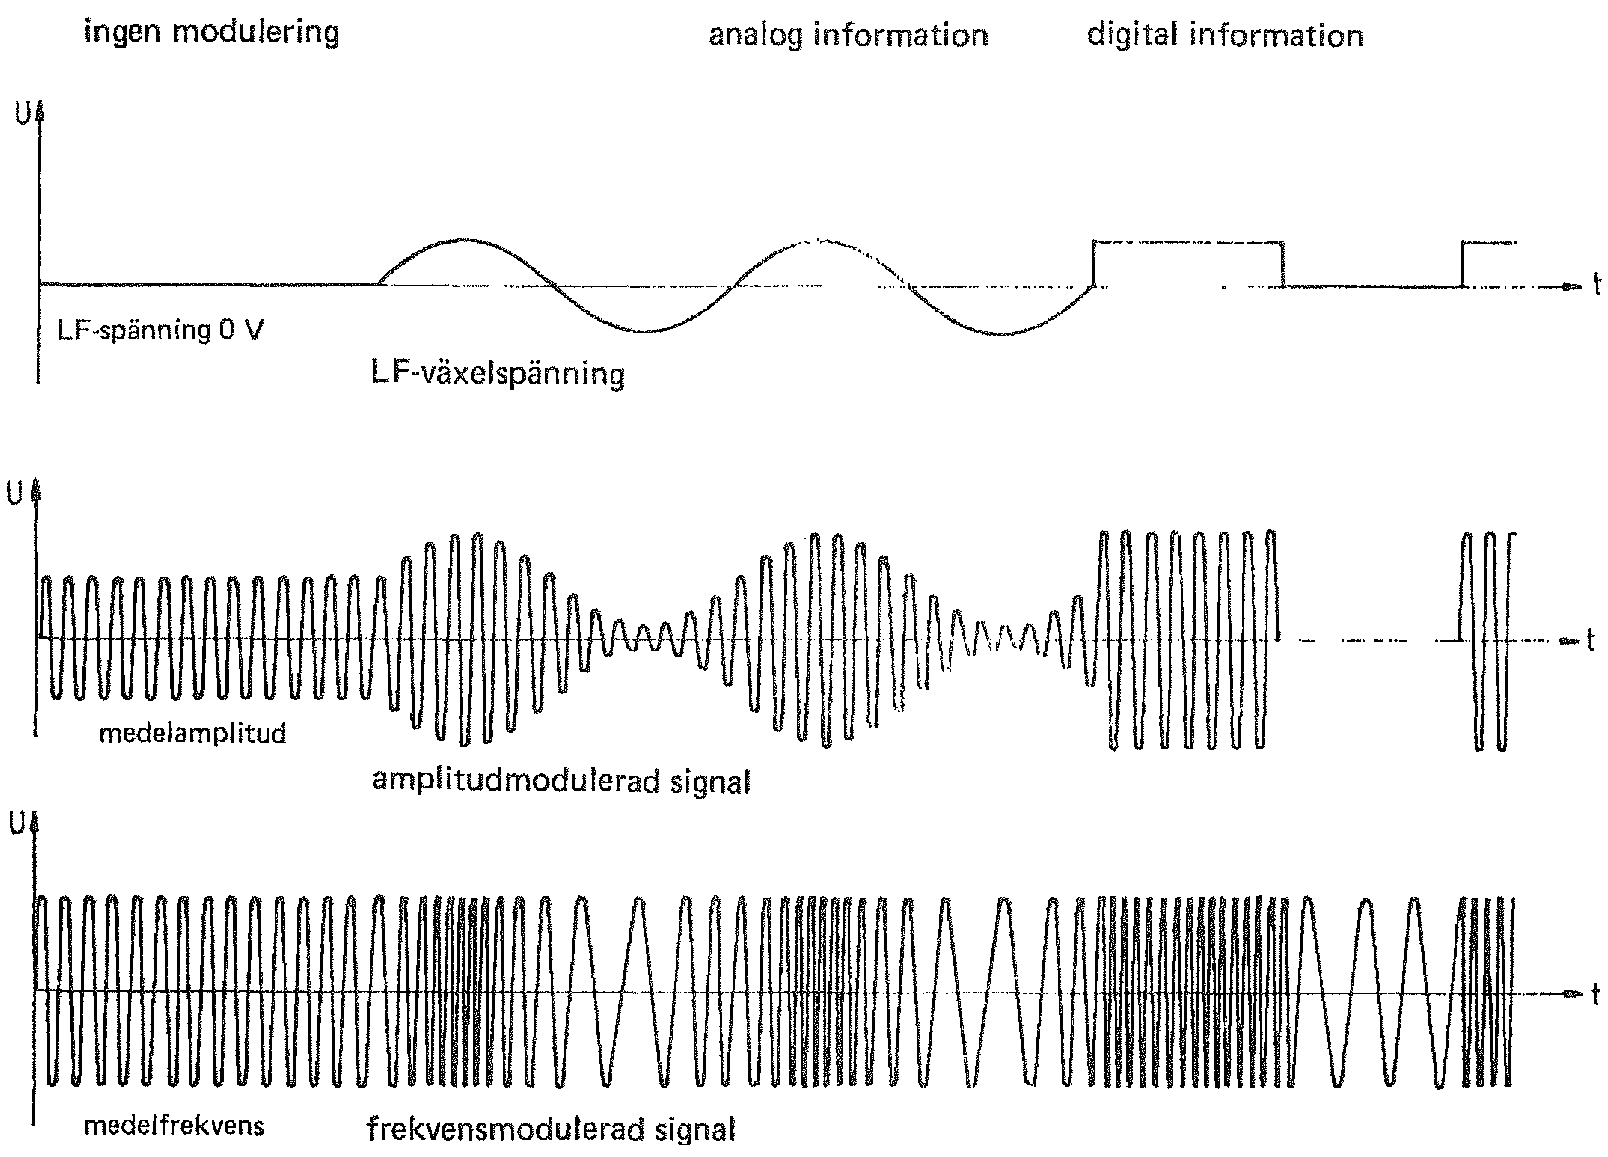
\includegraphics[width=14cm]{images/bild_2_1-22}
\caption{Modulerade signaler}
\label{fig:BildII1-22}
\end{center}
\end{figure*}

Bild \ref{fig:BildII1-22}.

En modulerad signal kännetecknas av dess amplitud, frekvens och fasläge.

Vid \emph{amplitudmodulation} påverkas huvudbärvågens amplitud, så att den i
varje tidpunkt motsvarar den modulerande signalens variation.

Vid \emph{frekvensmodulation} påverkas huvudbärvågens frekvens, så att den i
varje tidpunkt motsvarar den modulerande signalens variation.

Vid \emph{fasmodulation}, som är besläktad med frekensmodulation, påverkas i
stället för frekvensen huvudbärvågens fasläge i förhållande till en
referenssignal, så att fasläget i varje tidpunkt motsvarar den modulerande
signalens variation.

Frekvens- och fasmodulation liknar varandra och kan sammanfattas som
vinkelmodulation, eftersom fasvinkeln mellan bärvågens spänning och ström
varierar i båda fallen.

Vid \emph{pulsmodulation} används pulståg (korta upprepade bärvågspaket); t.ex.
pulsamplitud-, pulslängds-, pulsläges- och pulskodmodulation. Pulskodmodulation
används t.ex. vid samtidig överföring av flera telesamtal på samma linje,
bärvåg etc.

\subsection{Bandbredd vid olika sändningsslag}

Varje radiosändning tar upp plats omkring den nominella bärvågsfrekvensen -
tillsammans \emph{bandbredden}.

Radioamatören måste veta detta "platsbehov", främst för att inte sända utanför
de frekvensband som är tilldelade för amatörradioanvändning, men även för att
kunna umgås med annan trafik inom banden.

I alla sändningsslag ökar den använda bandbredden med ökad modulation. Eftersom
största \emph{frekvenseffektivitet} alltid skall eftersträvas så upptar en
sändare med kraftigare modulation än vad som behövs för en överföring, alltid
onödigt frekvensutrymme.

\subsection{Beskrivningskod för sändningsslagen}

Vid 1979 års radioförvaltningskonferens (WARC 79) i Geneve reviderades det
internationella radioreglementet (RR), som i huvudsak trädde i kraft 1982.
Däri ingår bl. a. ett nytt system för klassindelning och beteckning av sätten
att utsända information över radio m.m. Reglementet har reviderats senare, men
i detta stycke gäller det ännu.

Indelningen i sändningsslag behövs för att känneteckna utsändningarna, t. ex. i
frekvenslistor, författningar och föreskrifter. Indelningen är också av stort
värde vid teknisk beskrivning av apparater och system för radiokommunikation.

Emellertid används av många även äldre benämningar, vilka lever kvar i
litteraturen, i märkning av manöverdonen på sändare och mottagare o.s.v.

Dessa äldre benämningar är dock inte entydiga och skapar lätt missförstånd,
varför beskrivningskoden enligt WARC 79 bör användas för tydlighetens skull.

Här följer avkortade koder enligt WARC 79 för några av de sändningsslag, som
amatörer använder mest, samt för jämförelse även de benämningar som fortfarande
används jämsides (se vidare i Appendix E).

\begin{description}
\item[NON] Bärvåg utan modulerande signal. Ingen information.

\item[A1A] Bärvåg med dubbla sidband. En enda kanal med kvantiserad bärvåg.
Ingen modulerande underbärvåg. Telegrafi.

\emph{Även kallat nycklad bärvåg (CW).}

\item[A3E] Linjärt modulerad huvudbärvåg. Dubbla sidband. En enda kanal med
analog information. Telefoni.

\emph{Även kallat amplitudmodulation (AM).}

\item[J3E] Linjärt modulerad huvudbärvåg. Ett sidband med undertryckt bärvåg.
En enda kanal med analog information. Telefoni.

\emph{Även kallat enkelt sidband (Single Side Band - SSB).}

\item[F3E] Vinkelmodulerad bärvåg. Frekvensmodulering. En enda kanal med analog
information. Telefoni.

\emph{Även kallat frekvensmodulering (FM).}

\item[G3E] Vinkelmodulerad bärvåg. Fasmodulering. En enda kanal med analog
information. Telefoni.

\emph{Även kallat fasmodulering (PM).}
\end{description}

Såväl A1A, A3E som J3E är sändningsslag där amplituden moduleras. Därför är
termen \emph{amplitudmodulation} inte tillräcklig för att beskriva flera
likartade sändningsslag.

\subsection{Modulerande signaler}
\textbf{HAREC a.\ref{HAREC.a.1.7.1}\label{myHAREC.a.1.7.1}}

\subsubsection{Basband}

Basband är ett frekvensområde för en modulerande signal. Det finns ett basband
för alla slags modulerande signaler, vare sig de är analoga eller digitala. Det
kan finnas mer än ett basband i en komplett modulationsprocess. Till exempel är
en nycklad ton, som går till sändaren genom mikrofoningången, dess analoga
basband medan nycklingspulserna till tongeneratorn är dess digitala basband.

\begin{figure*}[ht]
\begin{center}
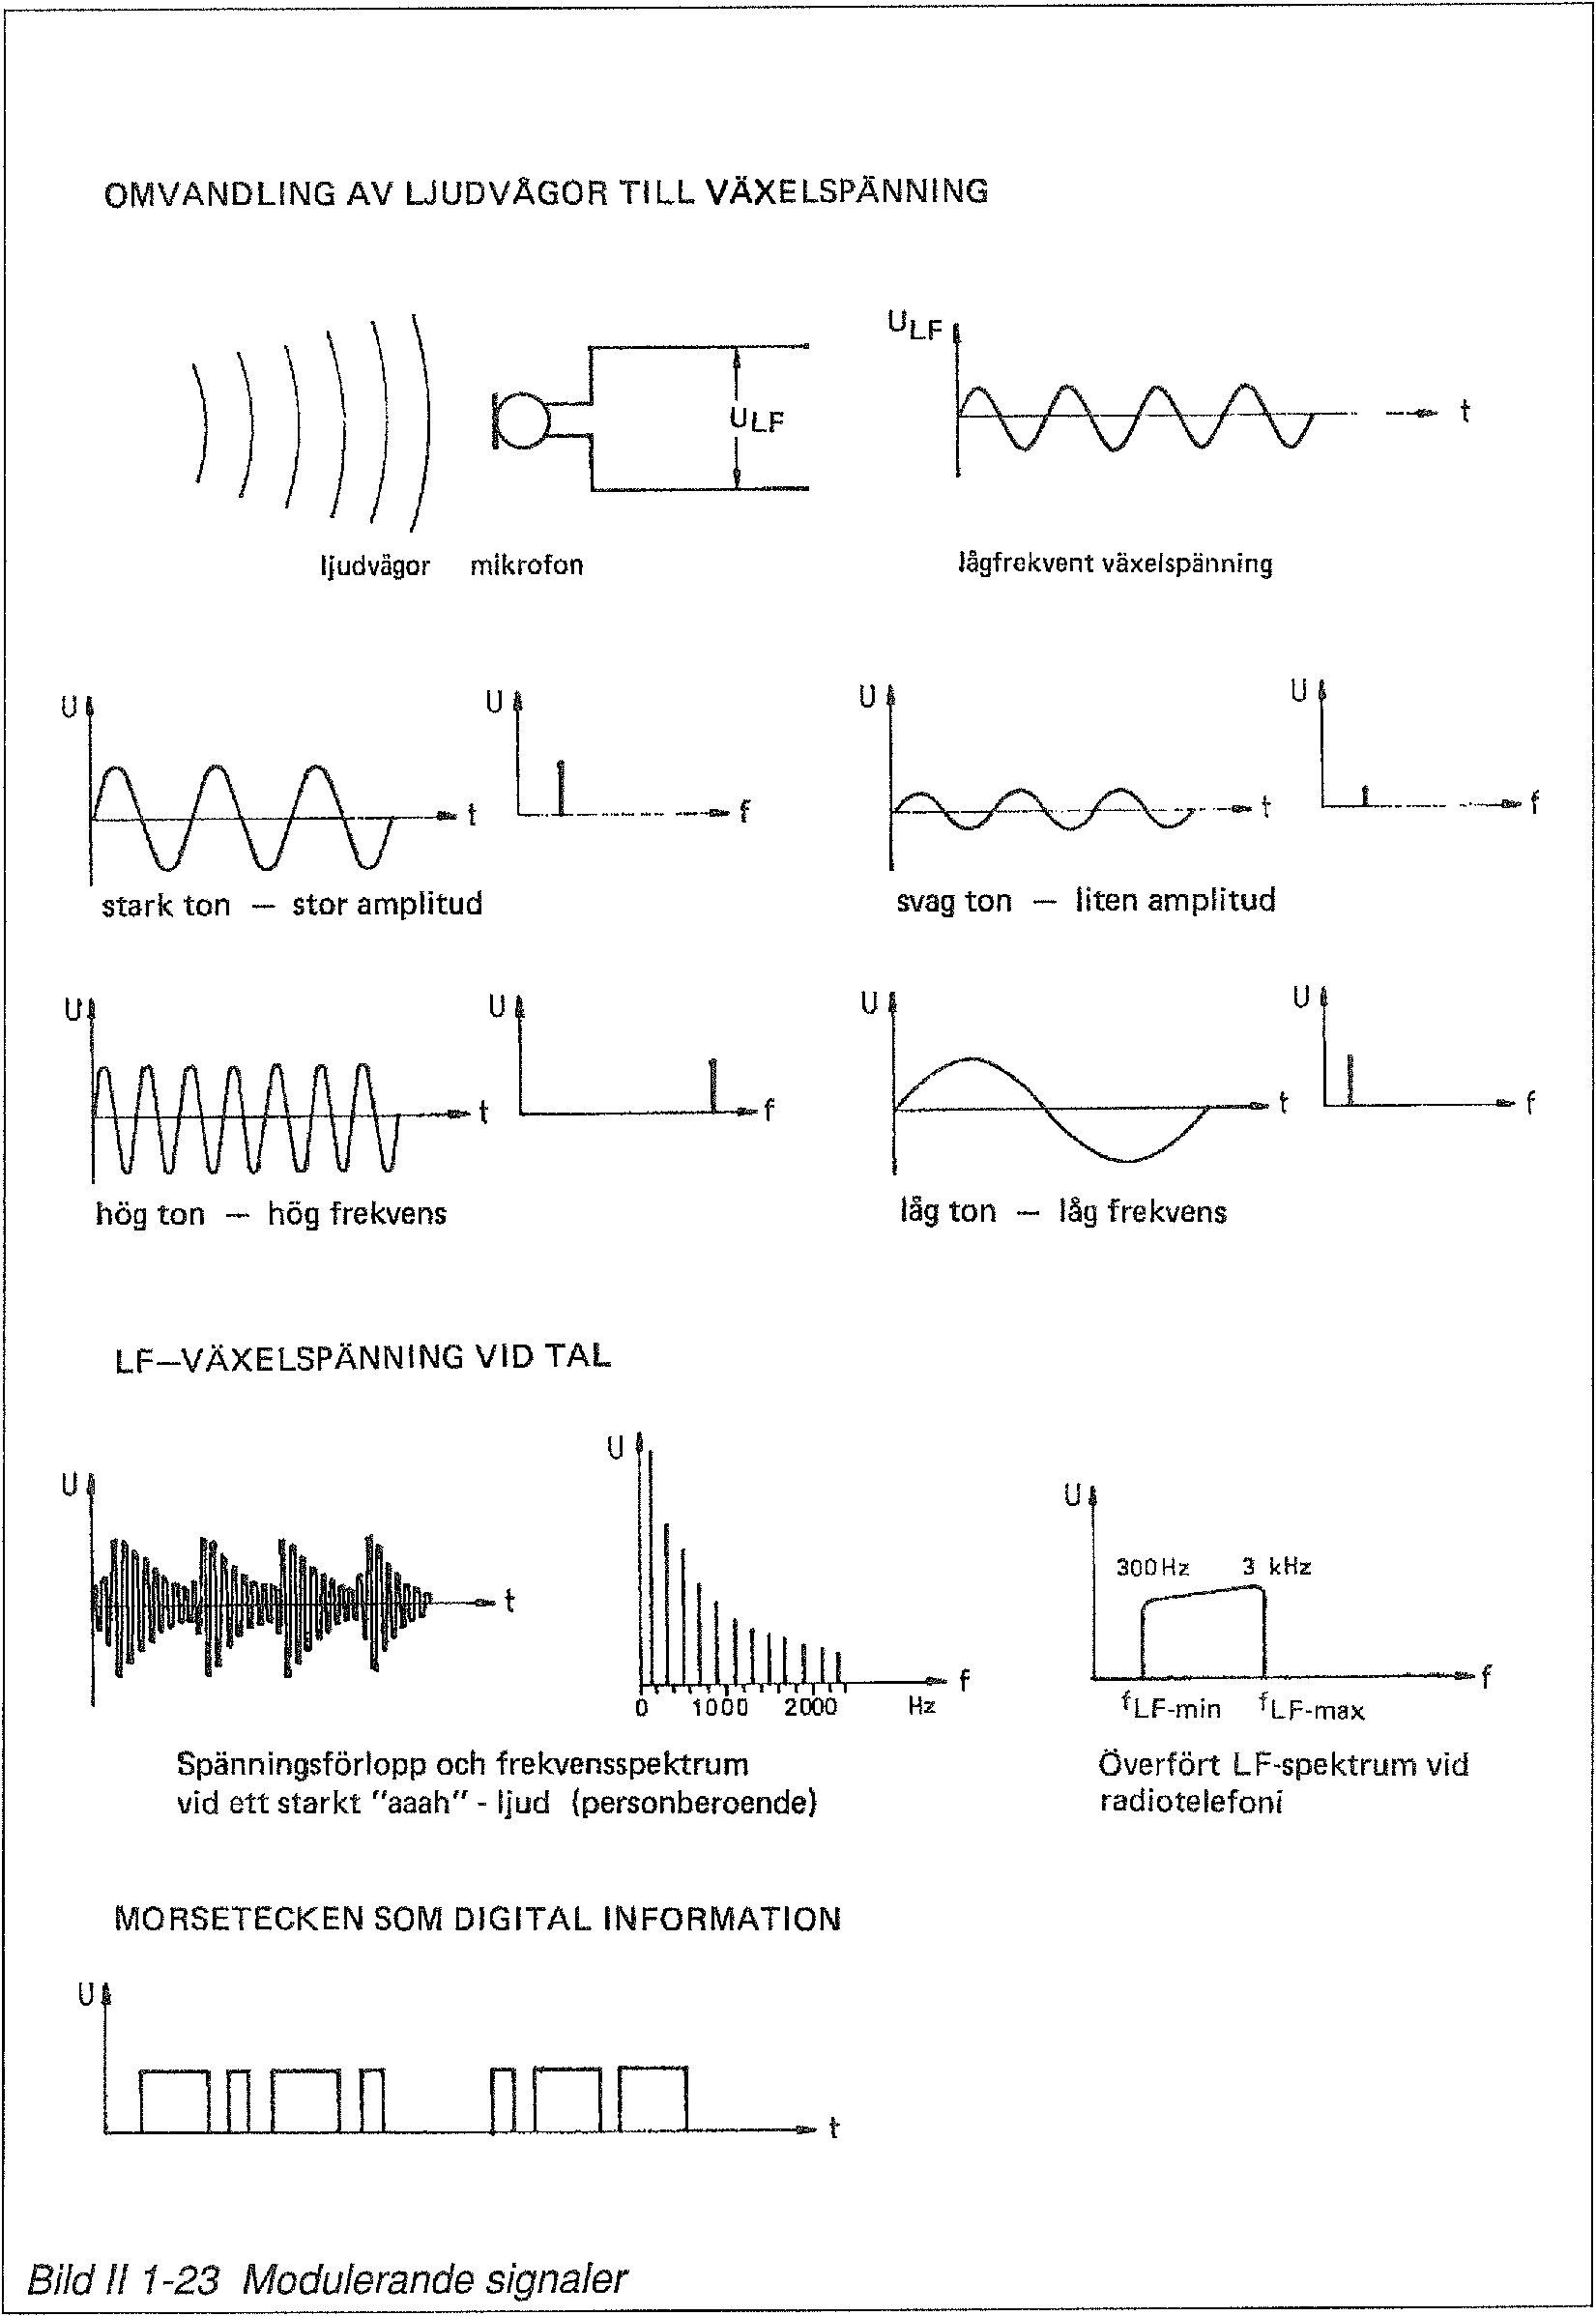
\includegraphics[width=14cm]{images/bild_2_1-23}
\caption{Modulerande signaler}
\label{fig:BildII1-23}
\end{center}
\end{figure*}

Bild \ref{fig:BildII1-23}.

Ett vanligt sätt att överföra information över radio är med telefoni, d.v.s.
tal.

Frekvensområdet 300-3000 Hz räcker för god förståelighet av tal. Dels är örat
känsligast inom det området och dels finns där den mesta energin i talet.

Mikrofonen tar upp de lufttrycksvariationer, som uppstår när man talar, och
omvandlar dem till elektriska svängningar. Svängningarna varierar mellan
positiva och negativa spänningsvärden.

\subsubsection{Försök}

\begin{enumerate}
\item Anslut en mikrofon till ett oscilloskop och studera spänningsförloppen
för olika slags ljud, toner, tal o.s.v. som funktion av tiden. På bilden är
dessa svängningar mycket förenklade, t.ex. sinusformade.

\item Anslut en högtalare och ett oscilloskop till en LF-generator, vars
frekvens och amplitud kan ändras. Lyssna på ljud med låg och hög frekvens samt
på svaga och starka ljud. En baston har låg frekvens och en diskantton har hög
frekvens. En svag ton har liten amplitud och en stark ton har stor amplitud.
\end{enumerate}

\subsection{Sändningsslaget A3E (även kallat AM)}
\textbf{HAREC a.\ref{HAREC.a.1.8.2}, a.\ref{HAREC.a.1.8.6b}, a.\ref{HAREC.a.1.8.7b}\label{myHAREC.a.1.8.2}\label{myHAREC.a.1.8.6b}\label{myHAREC.a.1.8.7b}}

\begin{figure*}[ht]
\begin{center}
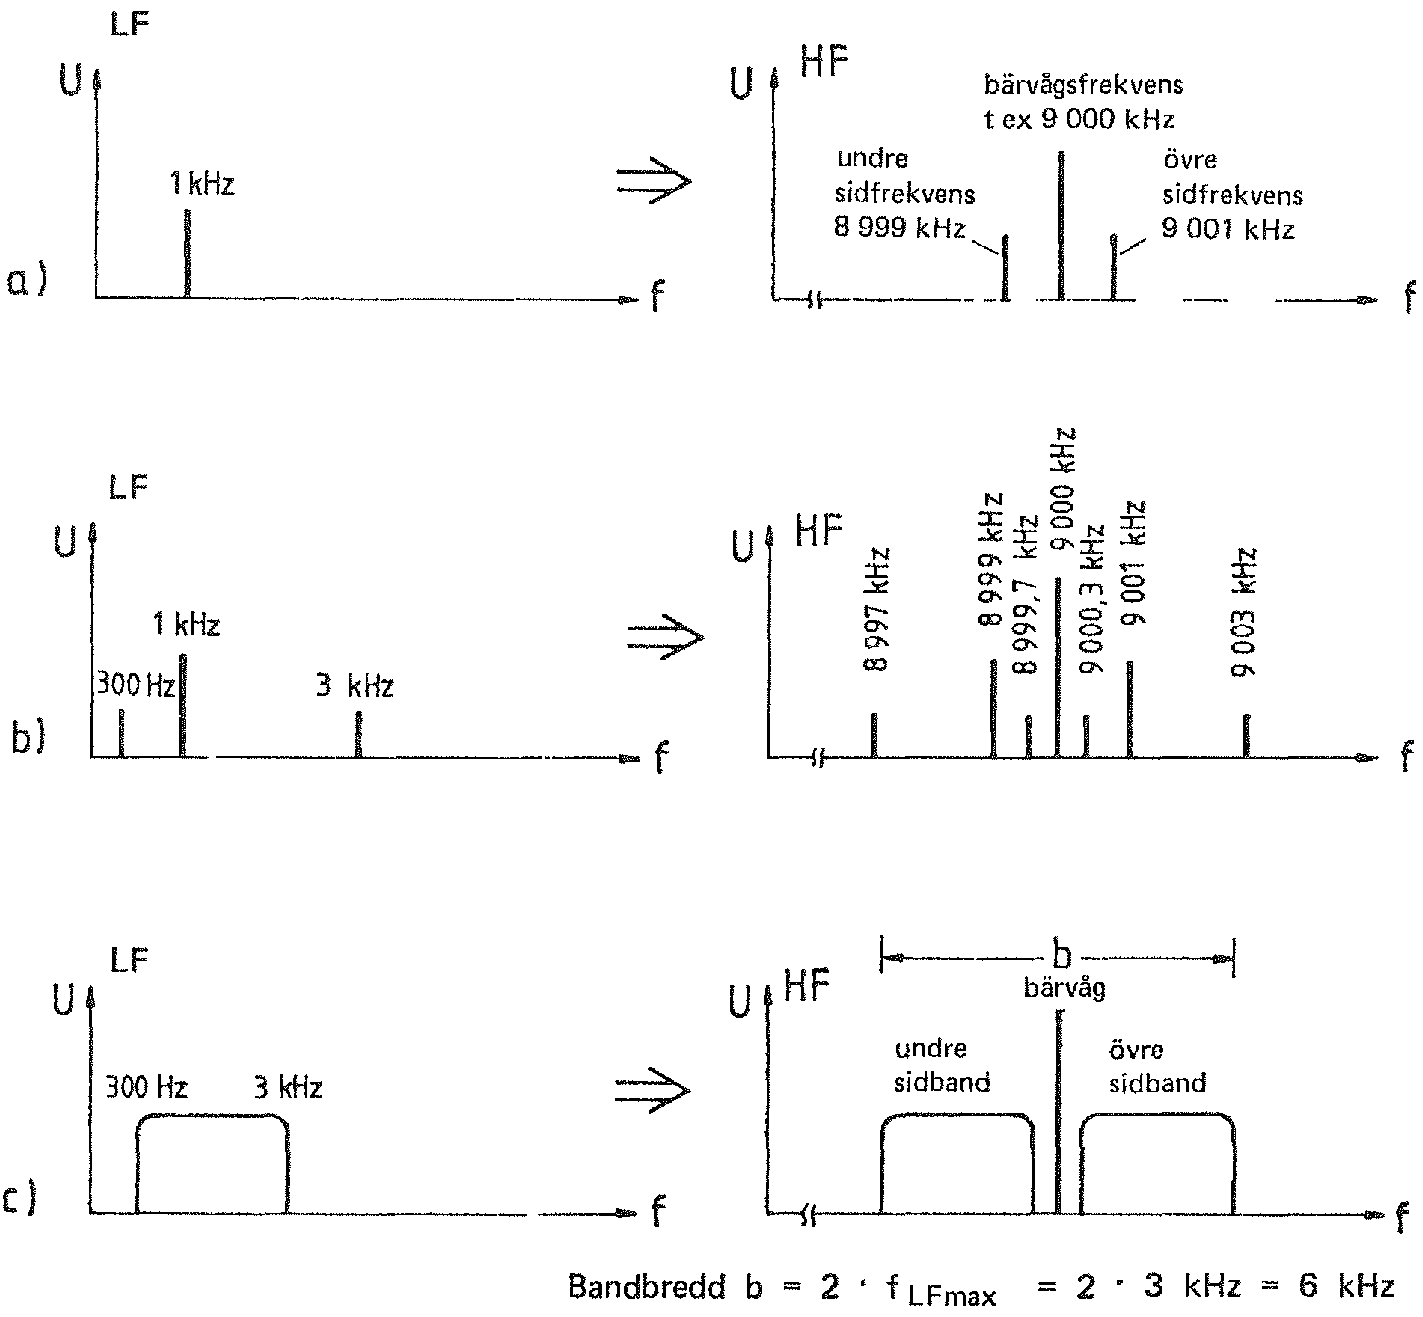
\includegraphics[width=14cm]{images/bild_2_1-24}
\caption{Sidband vid A3E-modulation}
\label{fig:BildII1-24}
\end{center}
\end{figure*}

Bild \ref{fig:BildII1-24}.

Bilden visar frekvensspektrum av en signal vid amplitudmodulation med

\begin{enumerate}[label=\alph*.,noitemsep]
\item en sinuston,
\item en blandning av tre sinustoner,
\item ett frekvensspektrum.
\end{enumerate}

\subsubsection{Försök}

Modulera en A3E-sändare med en 3 kHzsignal. Med en mottagare utrustad med ett
smalt filter för telegrafi, kan man urskilja och påvisa bärvågen och de båda
sidbanden.

\subsubsection{A3E-modulation med en ton}

\begin{figure*}[ht]
\begin{center}
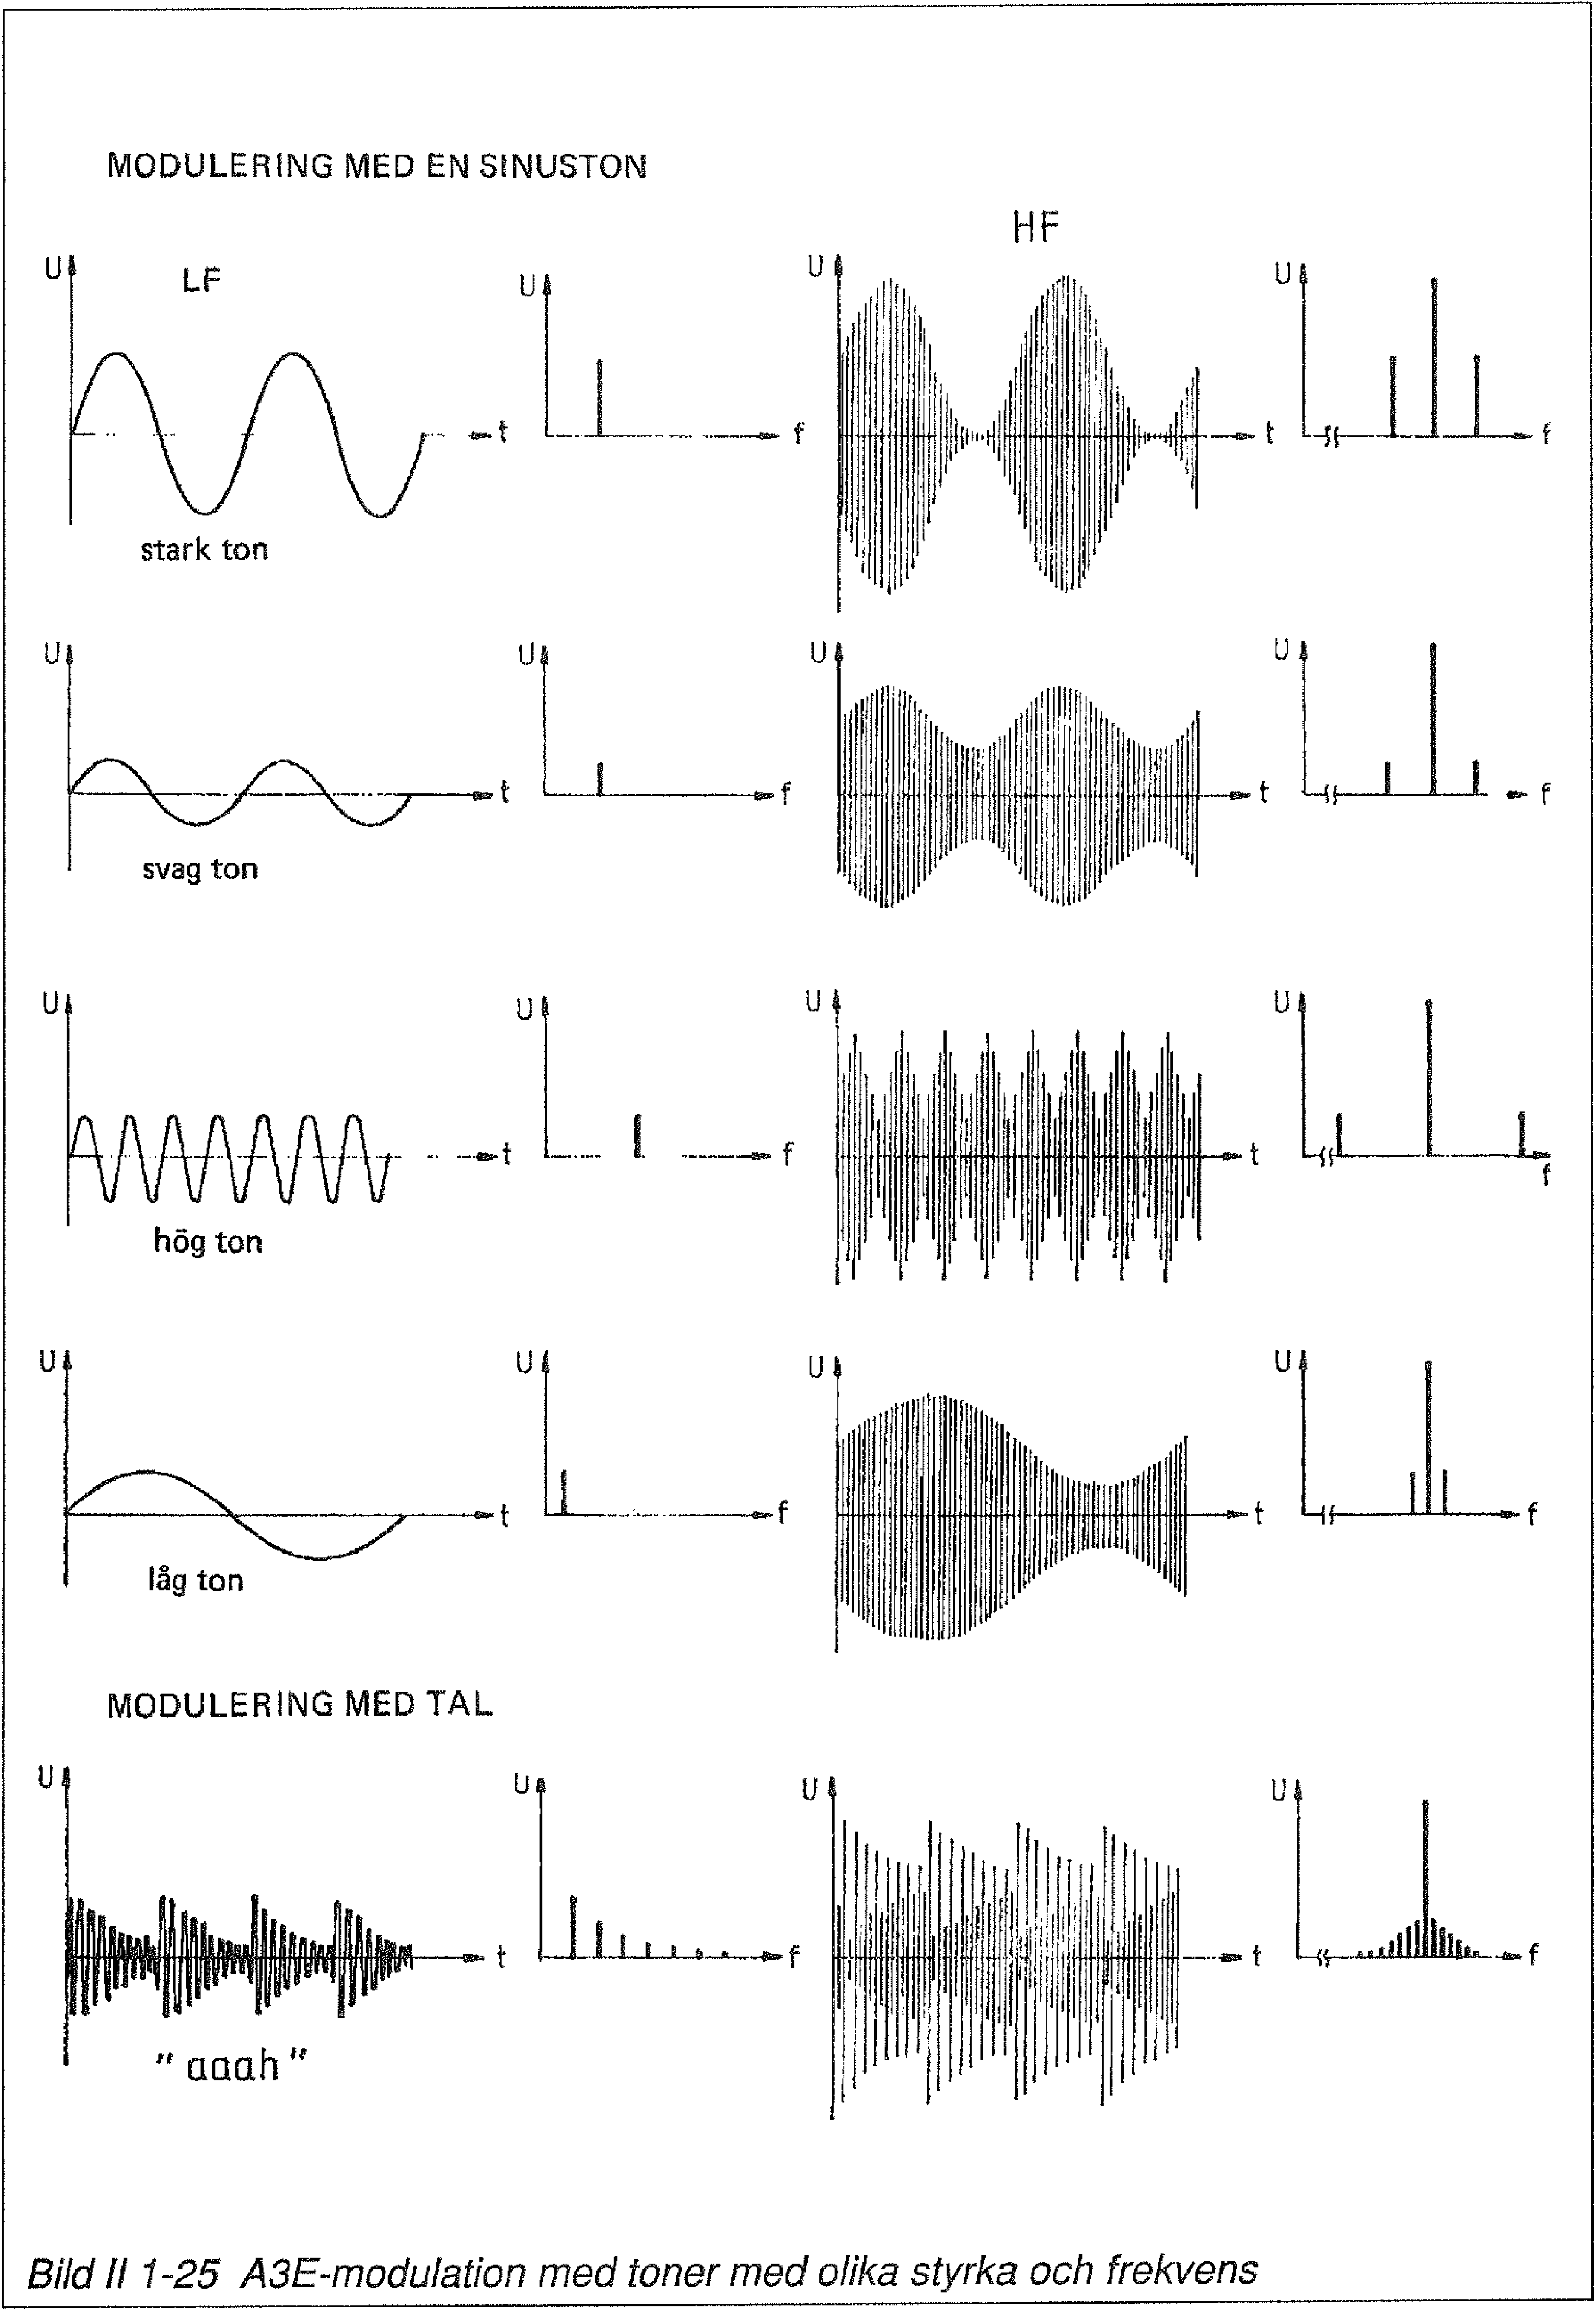
\includegraphics[width=14cm]{images/bild_2_1-25}
\caption{A3E-modulation med toner med olika styrka och frekvens}
\label{fig:BildII1-25}
\end{center}
\end{figure*}

Bild \ref{fig:BildII1-25}.

En omodulerad bärvåg har konstant amplitud. En amplitudmodulerad signal är i
grunden resultatet av svävning mellan frekvenser eller av icke linjär blandning
av frekvenser. När  bärvåg och basband blandas, så är särskilt tre
blandningsprodukter av intresse.

Dessa är

\begin{enumerate}[label=-,noitemsep]
\item bärvågen,
\item det lägre sidbandet (förkortat LSB) och
\item det övre sidbandet (förkortat USB).
\end{enumerate}

AM-signalen består således inte bara av bärvågsfrekvensen fHF utan även av övre
och nedre sidofrekvenser, vilka är summan och skillnaden av bärvågsfrekvensen
\(f_{HF}\) och den modulerande frekvensen \(f_{LF}\). Alltså \(f_{HF} + f_{LF}\)
(övre sidfrekvens) och skillnadsfrekvensen \(f_{HF} - f_{LF}\) (undre
sidfrekvens).

Eftersom tal inte bara omfattar en enda frekvens utan ett helt frekvensspektrum
(c:a 0.3 - 3 kHz), så uppstår inte bara två sidfrekvenser utan två sidband, det
lägre sidbandet (LSB, Lower Side Band) och det övre (USB, Upper Side Band).

LF-signalens frekvens bestämmer sidfrekvensens avstånd från bärvågen.
Bandbredden på en amplitudmodulerad signal med full bärvåg och två sidband är
dubbelt så stor som den högsta modulerande LFfrekvensen:

\(b= 2 \cdot f_{LFmax}\)

Om de modulerande LF-frekvenserna är mellan 0.3 och 3 kHz, så blir sändningens
totala bandbredd 6 kHz.

LF-signalernas amplitud påverkar sidbandens och sidfrekvensernas amplitud. Vid
maximal modulation (100 \% modulationsgrad) varierar signalamplituden mellan
noll och dubbla värdet av det för en omodulerad bärvåg.

Som mest kan vardera sidbandet överföra en fjärdedel så mycket effekt som
bärvågen, d.v.s. en sjättedel av den totalt utsända effekten. Då avger sändaren
dubbelt så stor medeleffekt som utan modulation. Toppeffekten (PEP,
Peak Envelope Power) är till och med fyra gånger så stor.

Slutförstärkaren och kraftförsörjningen måste dimensioneras för toppeffekten vid
full modulation eller att modulationsgraden anpassas så att överbelastning inte
sker.

\subsubsection{Fördelar med A3E-modulation}

En A3E-sändare är enkel jämfört med en J3E-sändare, vilken har en mer
komplicerad signalbehandling.

\subsubsection{Nackdelar med A3E-modulation}

Eftersom samma information finns i båda sidbanden och ingen finns i bärvågen,
så sänds effekten i bärvågen och ett av sidbanden ut till ingen nytta. I
talpauser sänds endast bärvågseffekten och till ingen nytta. Även
frekvensutrymme slösas bort. Då en annan, alltför närliggande sändares bärvåg
blandas med den egna, så alstras renstoner i mottagarna.

\subsection{Sändningsslaget A1A (även kallat CW)}
\textbf{HAREC a.\ref{HAREC.a.1.8.1}, a.\ref{HAREC.a.1.8.6a}, a.\ref{HAREC.a.1.8.7a}\label{myHAREC.a.1.8.1}\label{myHAREC.a.1.8.6a}\label{myHAREC.a.1.8.7a}}

\begin{figure*}[ht]
\begin{center}
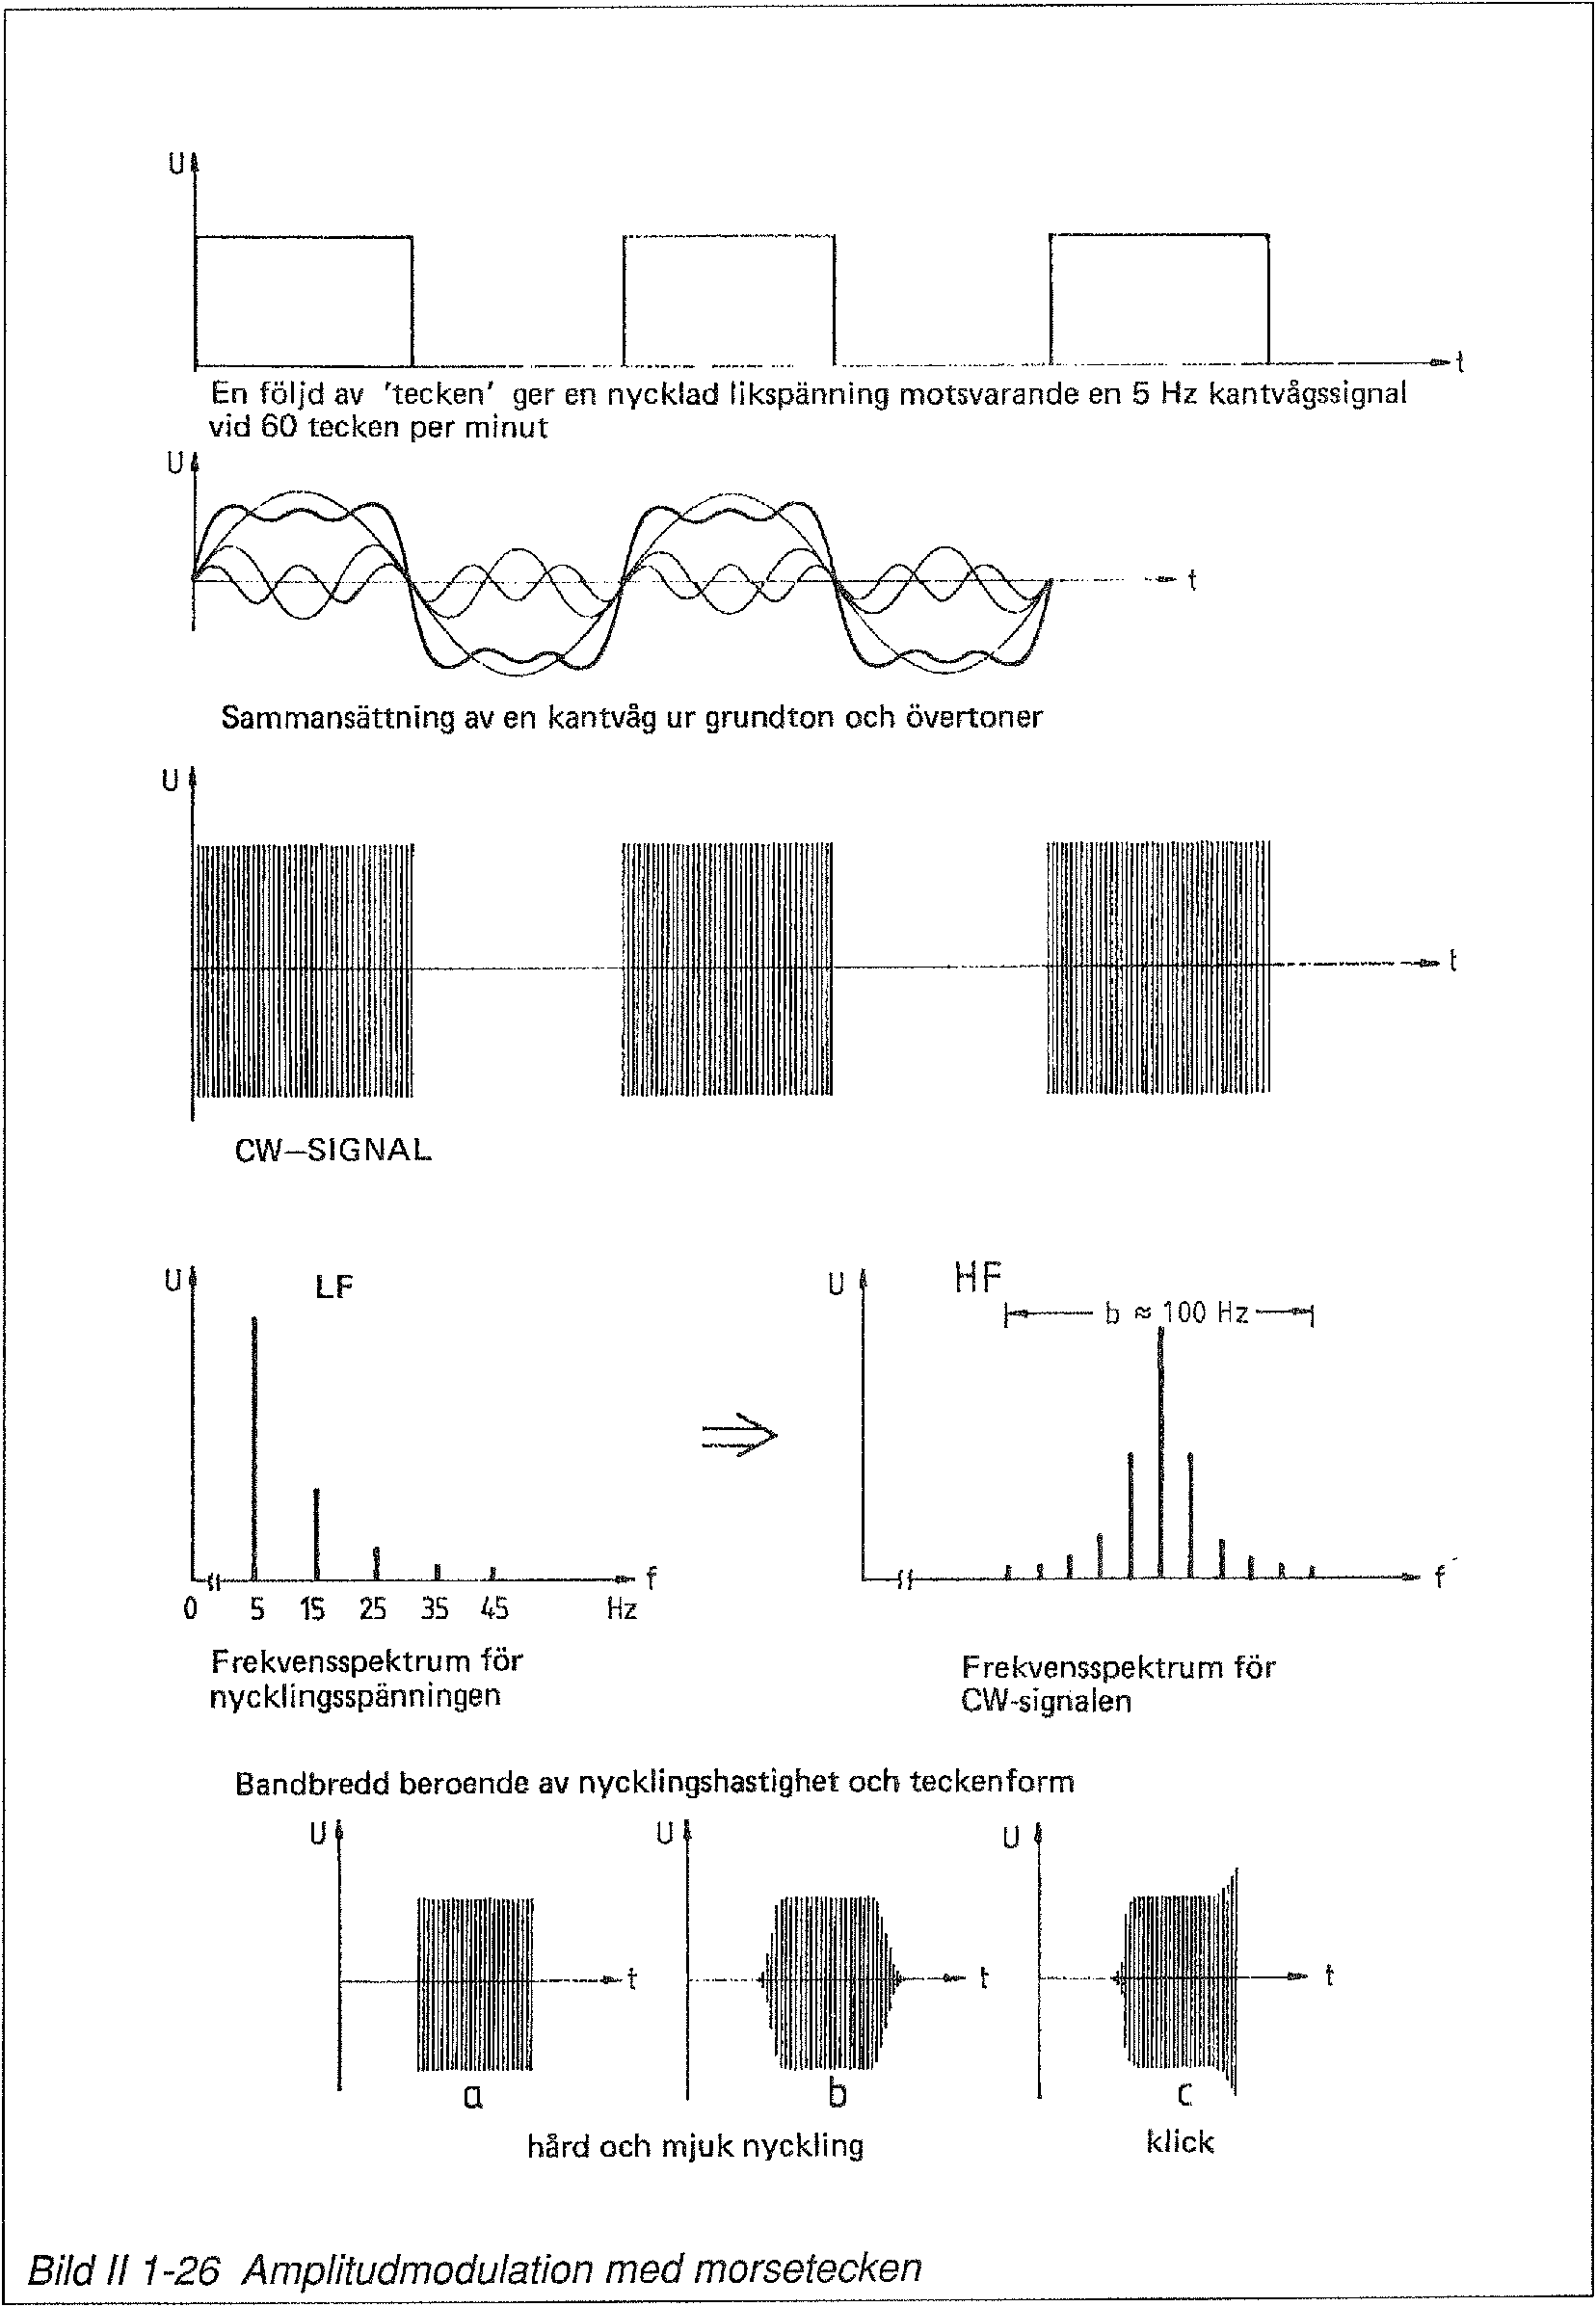
\includegraphics[width=14cm]{images/bild_2_1-26}
\caption{Amplitudmodulation med morsetecken}
\label{fig:BildII1-26}
\end{center}
\end{figure*}

Bild \ref{fig:BildII1-26}.

Man kan överföra meddelanden med morsetelegrafi på olika sätt. Det enklaste
sättet är att koppla in och ur sändarens bärvåg i takt med teckendelarna i
morsetecknen. Man kan kalla det för bärvågstelegrafi. Förfarandet kallas sedan
mycket länge även för CW (continous waves), vilket egentligen anger att
bärvågen svänger med konstant amplitud, om man bortser från att den nycklas.
Detta i motsats till de dämpade bärvågssvängningar som var fallet i sedan
mycket länge förbjudna s.k. gnistsändare.

Fastän en sändare "moduleras utan ton", har den en viss bandbredd. Det beror på
att den takt, som sändaren nycklas med, egentligen är en ton - låt vara med låg
frekvens. Antag att sändaren nycklas med en serie korta morsetecken. Vid
telegraferingshastigheten 60 tecken/minut alstrar bärvågspulserna en kantvåg
med frekvensen 5 Hz. Som tidigare beskrivits, består en sådan kantvåg av summan
av sinussignaler med frekvenserna 5 Hz, 15 Hz, 25 Hz, 35 Hz o.s.v.

Det innebär att det uppstår sidfrekvenser över och under bärvågens frekvens och
med ett avstånd till bärvågen av 5 Hz, 15 Hz, 25, 35Hz o.s.v ..
Telegrafisändaren har alltså liksom vid A3E en bandbredd, som dels står i
förhållande till nycklingshastigheten och dels till "kantigheten" på tecknen,
vilket bestämmer övertonshalten i bärvågen. Vid s.k. mjuk nyckling kan den 9:e
övertonen antas vara den högsta som uppfattas av en motstation. Med en
nycklingsfrekvens av 5 Hz blir bandbredden inte större än
\(2 \cdot 10 \cdot 5 = 100\ Hz\).

En hård (kantig) och snabb teckengivning ökar bandbredden och kan resultera i
att s.k. nycklingsknäppar kan uppfattas långt vid sidan om sändningsfrekvensen.
Ju hårdare nycklingen är, desto längre bort från bärvågsfrekvensen hörs
nycklingsknäpparna. Detta stör andra stationer.

Kännetecken för sändningsslaget A1A, telegrafi genom nycklad bärvåg:

Mycket liten bandbredd, extremt gott utnyttjande av sändareffekten, stor
överföringssäkerhet, lång räckvidd, enkla sändare.

\subsection{Sändningsslaget J3E (även kallat SSB)}
\textbf{HAREC a.\ref{HAREC.a.1.8.3c}, a.\ref{HAREC.a.1.8.6c}, a.\ref{HAREC.a.1.8.7c}\label{myHAREC.a.1.8.3c}\label{myHAREC.a.1.8.6c}\label{myHAREC.a.1.8.7c}}

\subsubsection{Princip}

Som sagts är det onödigt sända ut två sidband, eftersom båda innehåller samma
information.

Signaler med endast ett sidband och undertryckt bärvåg kan alstras på flera
sätt. Numera är den s.k. filtermetoden i särklass vanligast och den enda som
behandlas här.

\begin{figure*}[ht]
\begin{center}
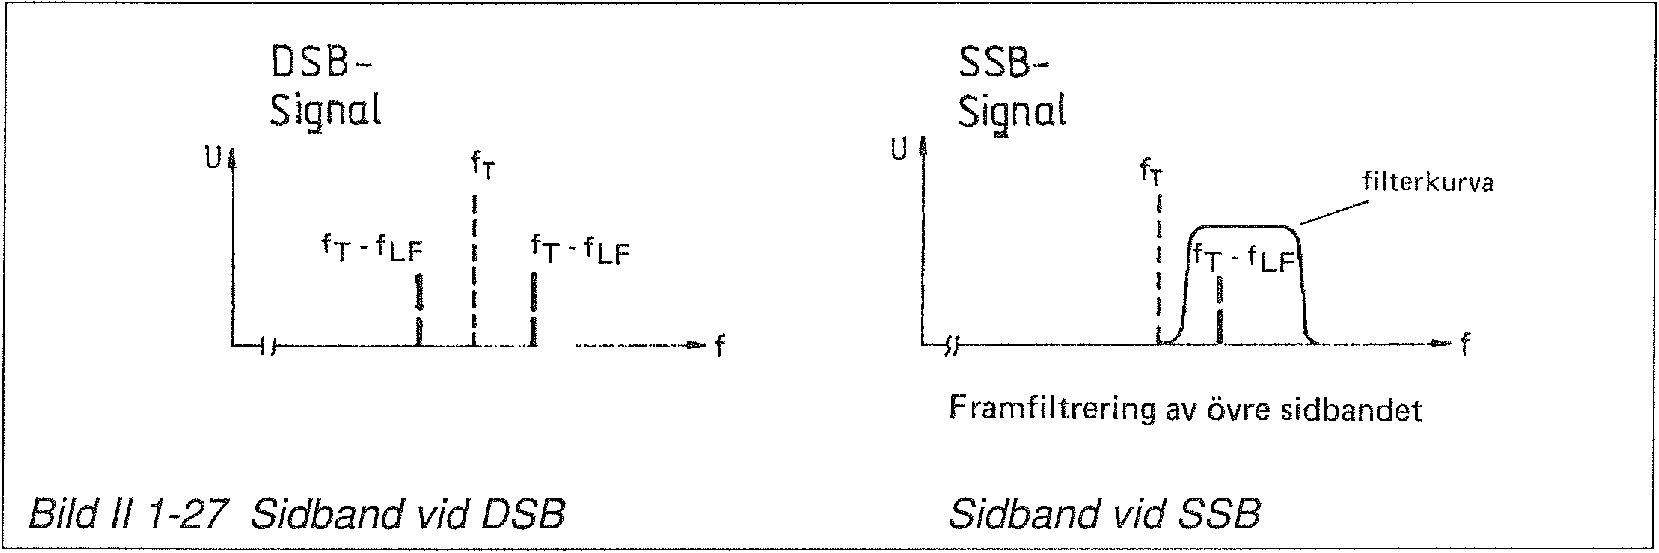
\includegraphics[width=14cm]{images/bild_2_1-27}
\caption{Sidband vid DSB}
\label{fig:BildII1-27}
\end{center}
\end{figure*}

Bild \ref{fig:BildII1-27}.

Med filtermetoden blandas HF- och LFsignalerna i en speciell blandare. Där
undertrycks båda dessa signaler medan blandningsprodukterna med deras summa-
och skillnadsfrekvenser blir kvar, d.v.s. det övre och nedre sidbandet.

Utsignalen från blandaren benämns DSBsignal (Double Side Band). Till skillnad
från i A3E-signalen saknas dock bärvågen i DSBsignalen. För att även
undertrycka det ena sidbandet före sändningen, så följs blandaren av ett
bandpassfilter med bandbredd och frekvensläge för avsett sidband.

Den signal som sänds ut innehåller därför endast ett sidband (Single Side Band).

\paragraph{Exempel}

\begin{figure*}[ht]
\begin{center}
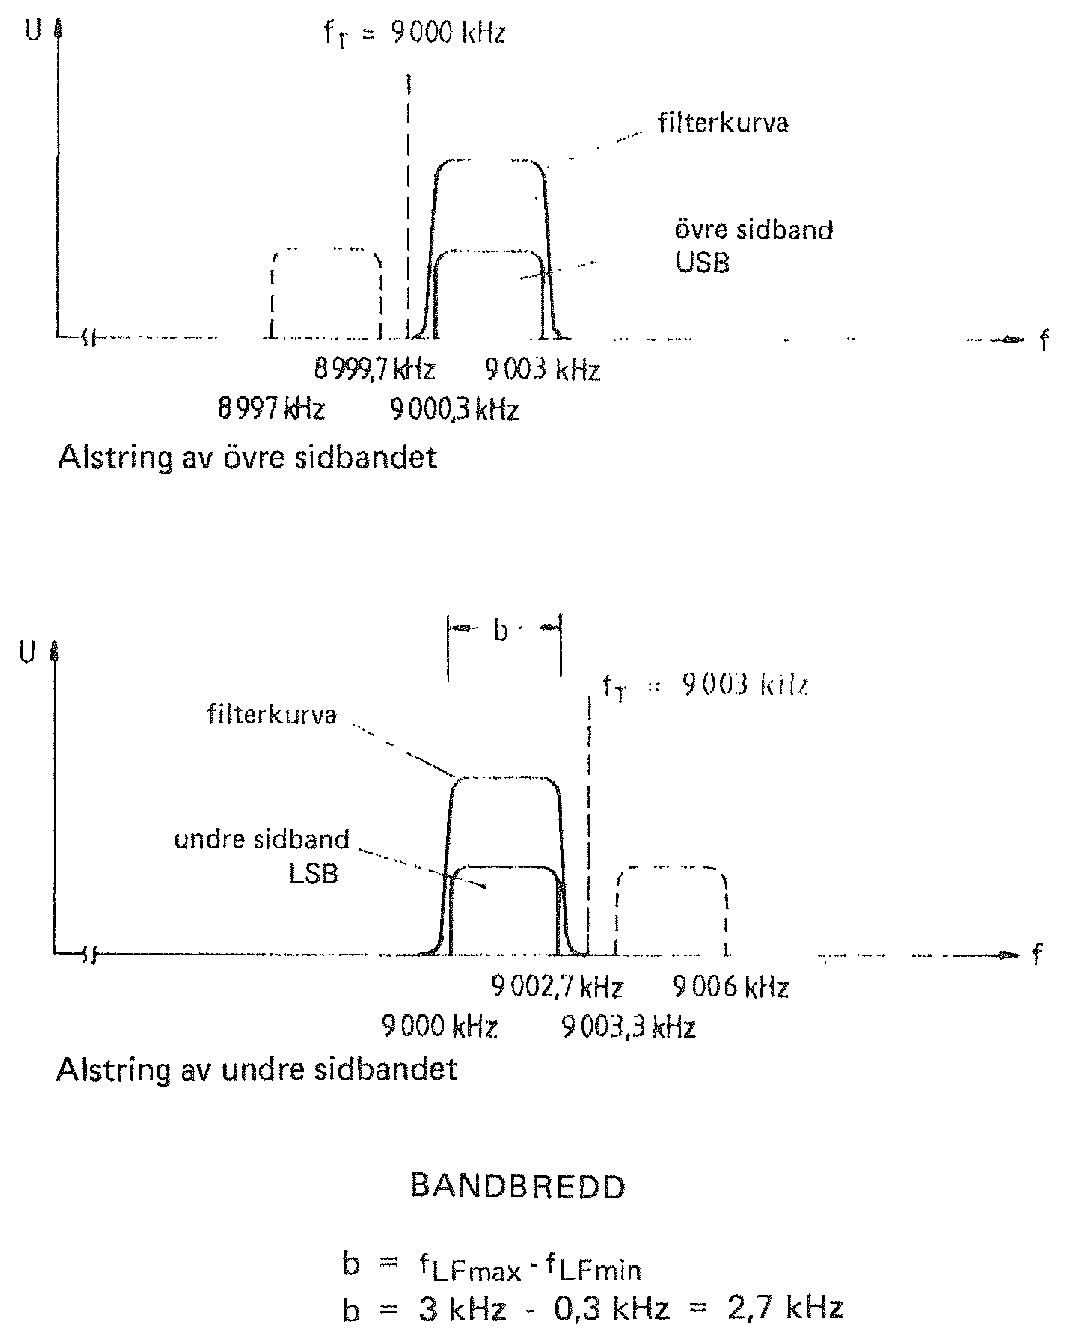
\includegraphics[width=14cm]{images/bild_2_1-28}
\caption{Sidbandsval vid SSB}
\label{fig:BildII1-28}
\end{center}
\end{figure*}

Bild \ref{fig:BildII1-28}.

Ett SSB-filter har ett passband av 9000.39003 kHz. Vid bärvågsfrekvensen 9000kHz
sträcker sig det övre sidbandet från 9003.39003 kHz och släpps igenom. Däremot
blir bärvågsfrekvensen undertryckt.

Det undre sidbandet 8997-8999.7 kHz faller utanför filtrets passband och blir
också undertryckt.

Skall däremot det undre sidbandet kunna passera igenom samma filter, så måste
bärvågsfrekvensen höjas med 3 kHz, alltså till 9003 kHz. Då faller det undre
sidbandet, 9002.7-9000.0 kHz inom filtrets passband.

Det övre sidbandet 9003.3-9006.0 kHz faller nu utanför passbandet och blir
undertryckt.

\begin{figure*}[ht]
\begin{center}
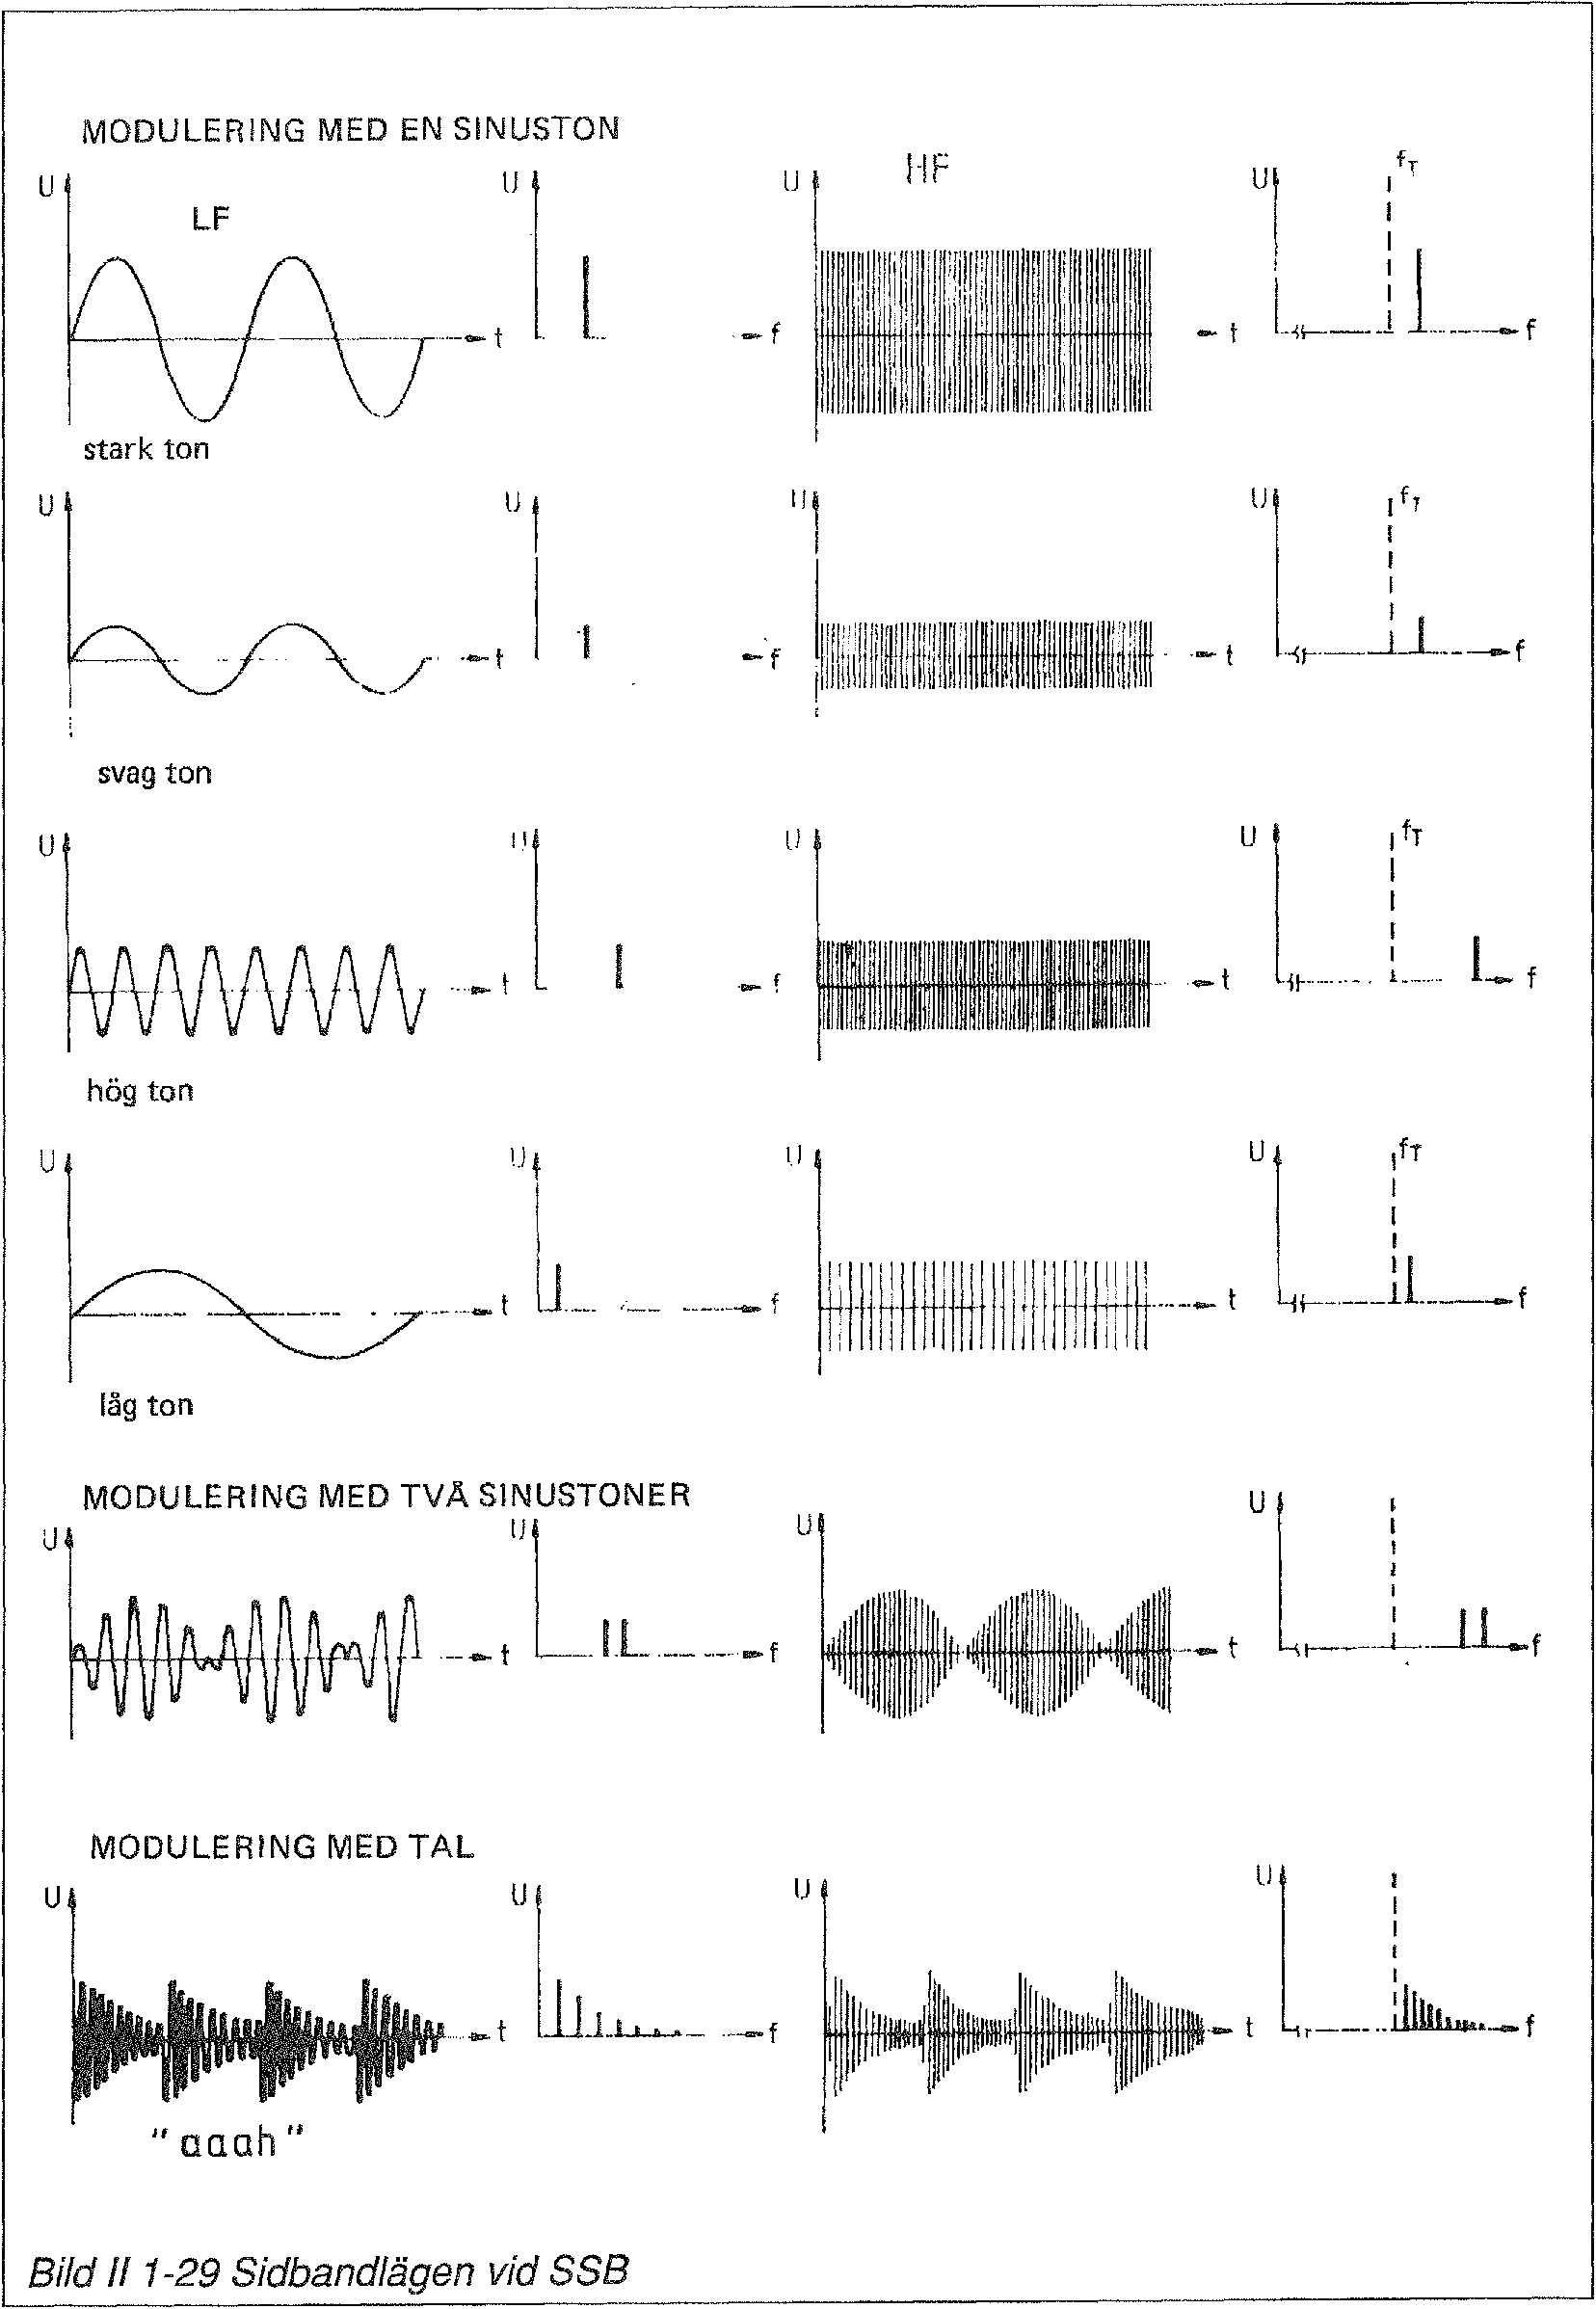
\includegraphics[width=14cm]{images/bild_2_1-29}
\caption{Sidbandlägen vid SSB}
\label{fig:BildII1-29}
\end{center}
\end{figure*}

Bild \ref{fig:BildII1-29}.

LF-signalens amplitud bestämmer amplituden på sidfrekvensen.

LF-signalens frekvens bestämmer sidfrekvensens avstånd från bärvågsfrekvensen
(bärvågen undertryckt).

Bandbredden på den utsända signalen är skillnaden mellan högsta och lägsta
modulerande frekvens i signalen:

t.ex. \(b = 3kHz - 0.3 kHz = 2.7 kHz\)

\subsubsection{Fördelar med J3E-modulation}
Bra verkningsgrad vid J3E-modulation jämfört med vid A3E-modulation
(traditionell AM). Effekten i det utsända sidbandet motsvarar den i ett av
sidbanden vid A3E. Hela den utsända effekten finns alltså i ett enda sidband,
som överför hela informationen.

I sändningspauserna sänds ingen effekt ut. Bandbredden är mindre än hälften av
den vid A3E. Vid mottagning av en J3E-sändning (SSB) är det mindre besvär med
interferenstoner från J3E-sändningar på närliggande frekvenser, eftersom ingen
bärvåg och endast ett sidband sänds ut.

\subsubsection{Nackdelar med J3E-modulation}
J3E-modulation medför mera komplicerade apparater, både för mottagning och
sändning. En J3E-signal blir förvrängd och hörs i fel tonläge, om mottagaren
inte är inställd på exakt rätt frekvens.

\subsection{Vinkelmodulation}
\textbf{HAREC a.\ref{HAREC.a.1.8.3b}, a.\ref{HAREC.a.1.8.6d}\label{myHAREC.a.1.8.3b}\label{myHAREC.a.1.8.6d}}

Termen vinkelmodulation är samlingsnamnet för frekvensmodulation (FM) och
fasmodulation (PM). Ofta sägs utrustningar vara för frekvensmodulation, när de
antingen är för frekvens- eller fasmodulation. Det finns alltså skillnader och
likheter mellan dessa system, vilka emellertid inte är oberoende av varandra,
eftersom frekvensen i en signal inte kan varieras utan att fasen också
varieras, och vice versa.

Hur effektiv kommunikationen då är, beror mest på mottagningsmetoderna. I båda
fallen uppfattas ändringar i den mottagna signalens frekvens och fasläge.
Amplitudändringar uppfattas däremot inte. De flesta störningar - särskilt
pulserande sådana som från tändningssystem - kommer att därför att skiljas bort.

För att effektivt utnyttja fördelarna med vinkelmodulation, antingen det är
frekvenseller fasmodulation, behövs tillräckligt frekvensutrymme. Det innebär
att främst högre frekvensband kommer i fråga.

\subsection{Frekvensmodulation (även kallat FM)}
\textbf{HAREC a.\ref{HAREC.a.1.8.3b}\label{myHAREC.a.1.8.3b}}

\begin{figure*}[ht]
\begin{center}
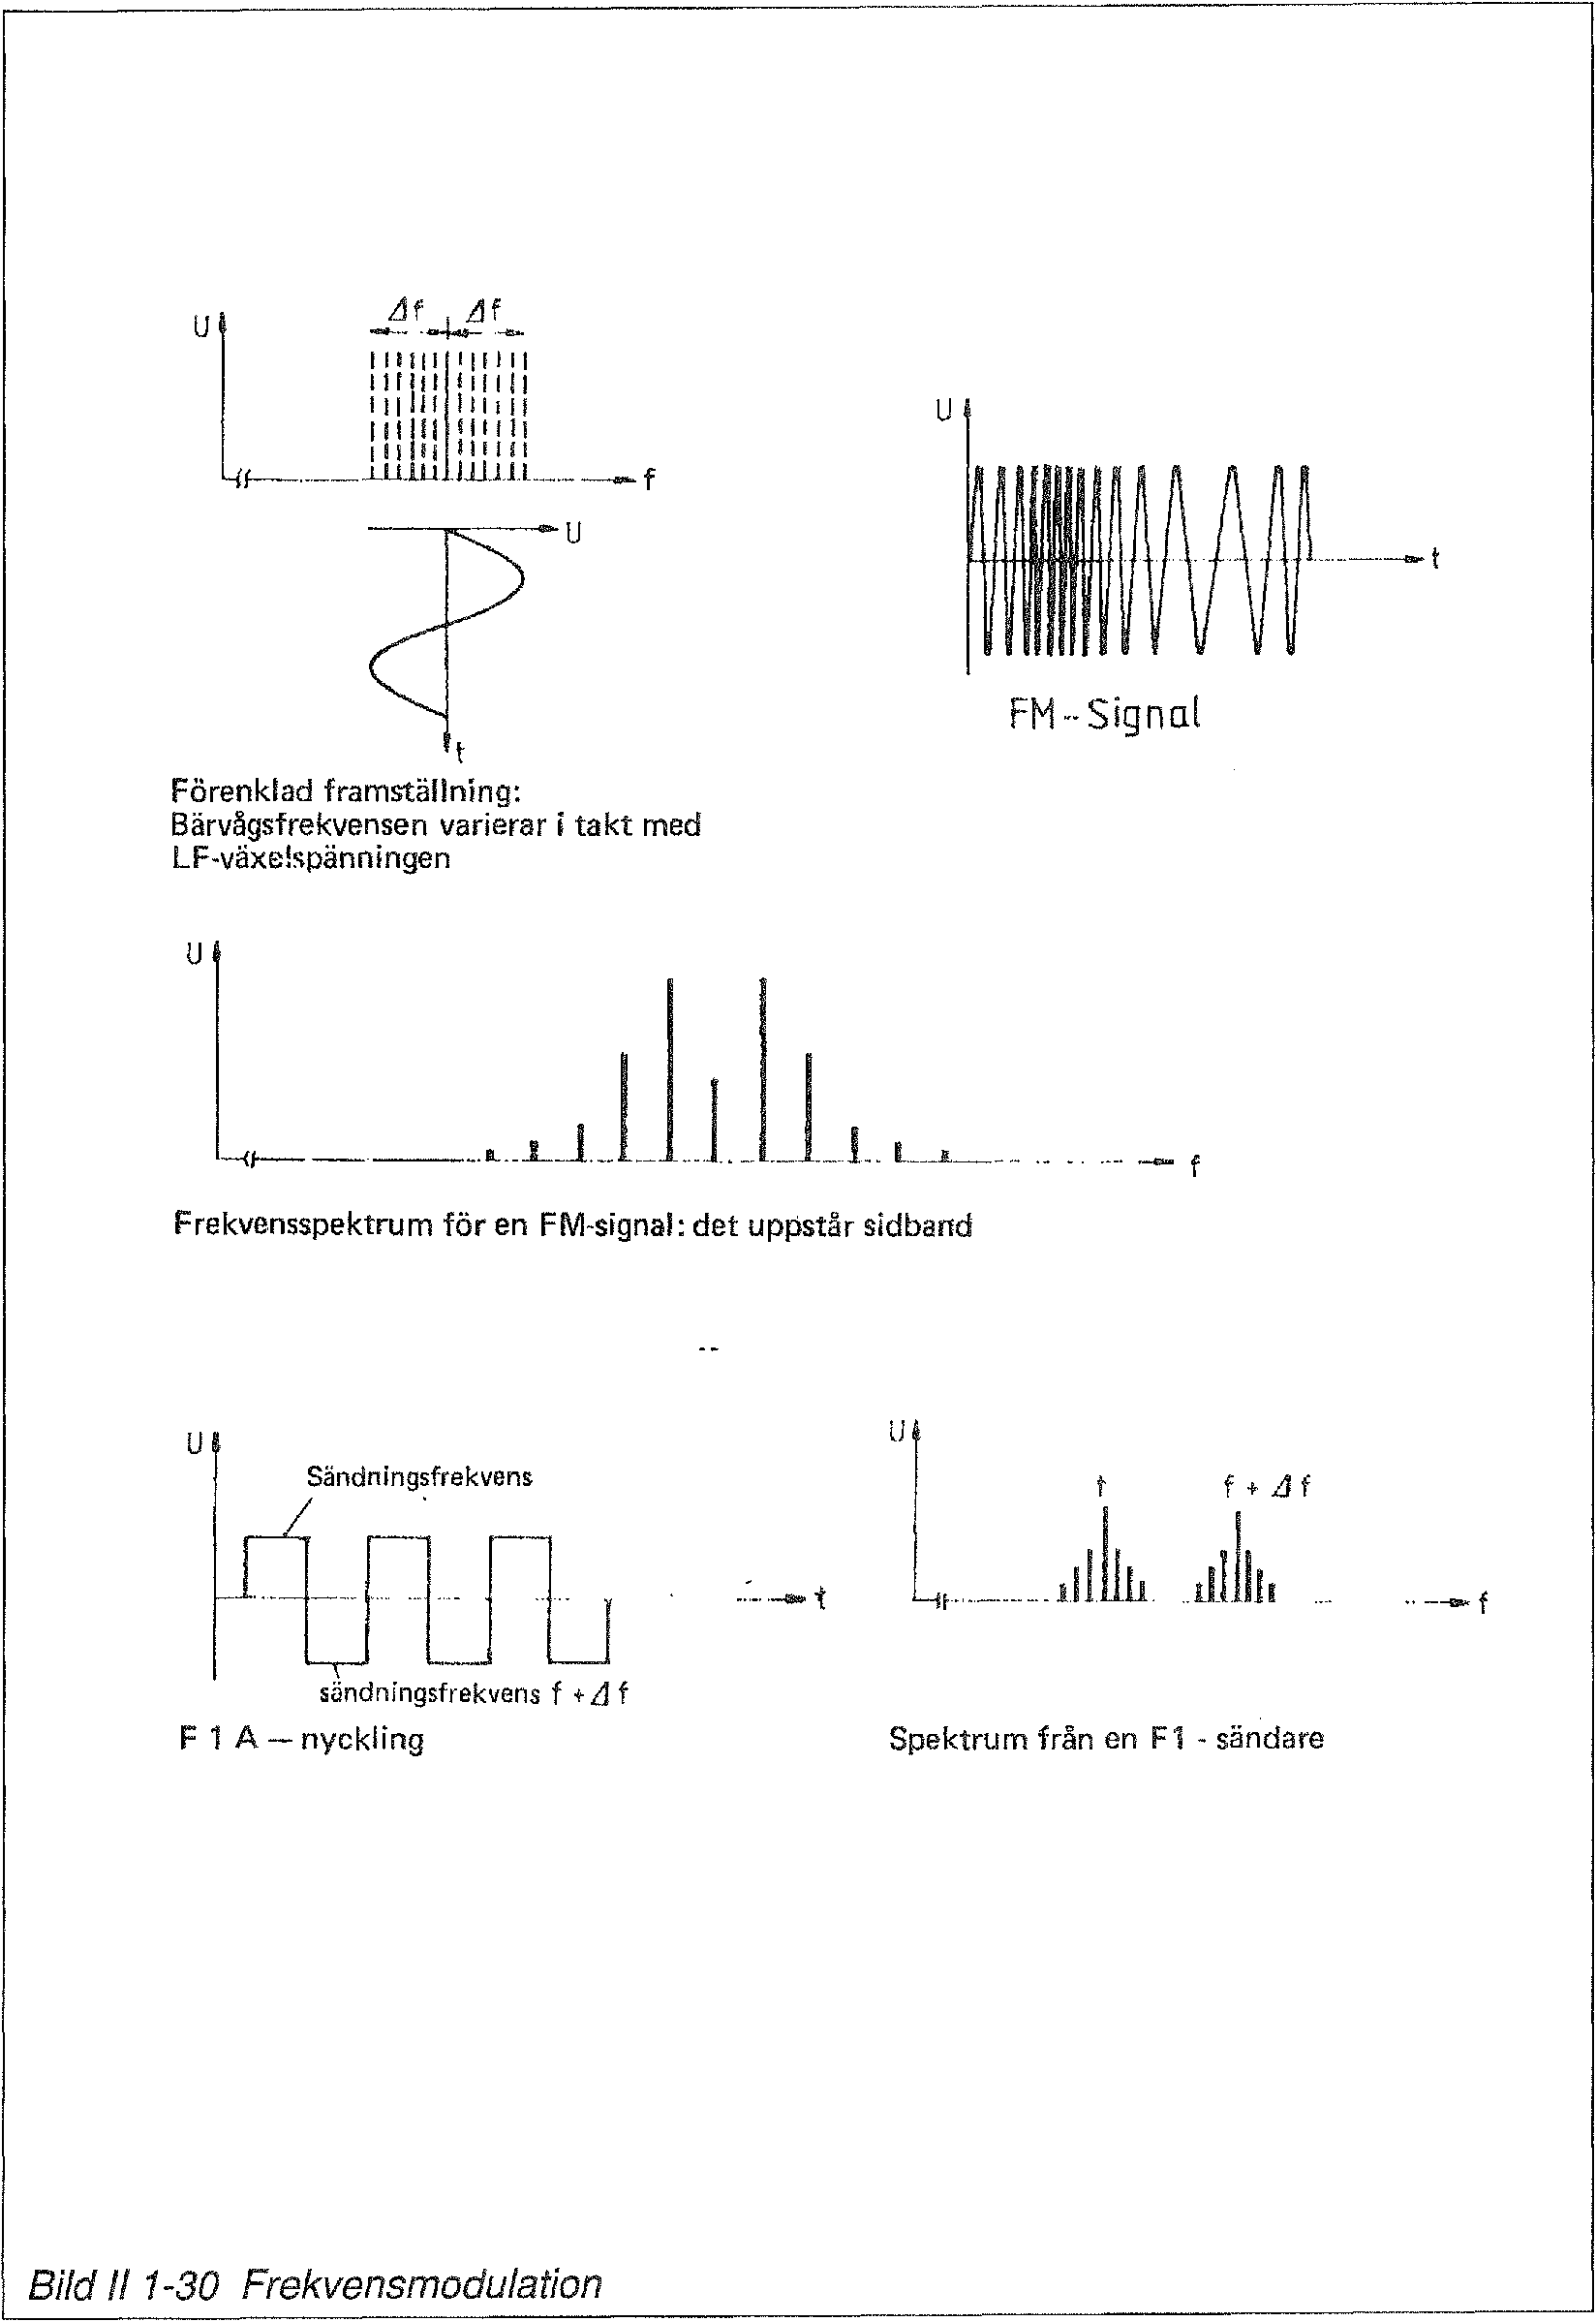
\includegraphics[width=14cm]{images/bild_2_1-30}
\caption{Frekvensmodulation}
\label{fig:BildII1-30}
\end{center}
\end{figure*}

Bild \ref{fig:BildII1-30} (överst och i mitten).

Vid frekvensmodulation varierar bärvågens frekvens i takt med den modulerande
signalens amplitud och polaritet. På bilden ökar bärvågens frekvens när den
modulerande signalen är positiv (första halvperioden) och minskar när den
modulerande signalen är negativ (andra halvperioden). Bilden visar att
perioderna i den modulerade bärvågen tar kortare tid (har högre frekvens), när
den modulerande signalen är positiv, och mertid (har lägre frekvens) när den
modulerande signalen är negativ. Bärvågen kommer alltså att pendla omkring ett
medelvärde, d.v.s. vara frekvensmodulerad.

Frekvensavvikelsen \(\Delta f\) (deviationen) från bärvågens vilafrekvens är
vid varje tillfälle proportionell till den modulerande signalens amplitud.
Sålunda är deviationen liten när den modulerande signalens amplitud är liten
och störst när amplituden når sitt toppvärde, antingen amplituden är positiv
eller negativ. Vid en modulationsfrekvens av 300 Hz varierar bärvågsfrekvensen
300 gånger per sekund, vid 3kHz - 3000 gånger per sekund.

Likspänningsnivåer kan överföras med FM, eftersom en motsvarande
frekvensavikelse kan framställas.

Bilden visar också vad som oftast sägs, att bärvågsamplituden inte ändras av
modulationen. Detta är emellertid bara delvis sant, eftersom såväl
bärvågsamplitud som sidbandsamplitud varierar med modulationsindex, vilket
förklaras nedan.

\subsubsection{Sidbanden vid vinkelmodulation}

Vid AM produceras endast ett sidbandspar med samma inne hål!, ett över och ett
under bärvågsfrekvensen. Vid vinkelmodulation, både vid FM och PM, produceras
däremot flera sidbandspar över och under bärvågsfrekvensen. Dessa sidband
uppträder på multiplerna av varje modulerande frekvens. Vid basband med samma
frekvensomfång har därför en vinkelmodulerad signal större bandbredd än en
AM-signal.

Vid vinkelmodulation beror antalet sidband på sambandet mellan den modulerande
frekvensen, frekvensdeviationen och modulationsindex.

\subsubsection{Bandbredden vid vinkelmodulation}

Bild \ref{fig:BildII1-30} (nederst).

Vi gör tankeexperimentet att en FM-sändare moduleras med en fyrkantvåg.
Frekvensen kommer då att hoppa växelvis mellan frekvenserna \(f\) och
\(f + \Delta f\). Sättet kallas FSK (frekvensskiftnyckling) och används t.ex.
vid sändning av radiofjärrskrift (RTTY, AMTOR, Paketradio etc.).

Vi föreställer oss två sändare, som sänder varannan gång, varav den ena sänder
frekvensen \(f\) och den andra sänder \(f + \Delta f\). Båda sändarnas
HF-signaler kommer då att bilda ett frekvensspektrum, som förutom \(f\) och
\(f + \Delta f\) även innehåller sidfrekvenser.

Bredden på detta spektrum beror bl. a. på nycklingsfrekvensen. Eftersom en
fyrkantvåg innehåller summan av dess grundfrekvens och övertoner, kommer alla
dessa toner att modulera vardera sändaren. De högsta modulerande
LF-frekvenserna alstrar sidfrekvenserna längst ut från vilofrekvensen.
LF-signalens frekvensspektrum påverkar alltså HF-signalens bandbredd.

Spektrum nederst i bilden är en förenklad framställning av
frekvensskiftnyckling.

Vid modulation med en sinussignal istället för med en fyrkantsignal, uppstår ett
frekvensspektrum som på överst i bilden.

\paragraph{Frekvensdeviation och modulationsindex}
\textbf{HAREC a.\ref{HAREC.a.1.8.4}\label{myHAREC.a.1.8.4}}

\begin{figure*}[ht]
\begin{center}
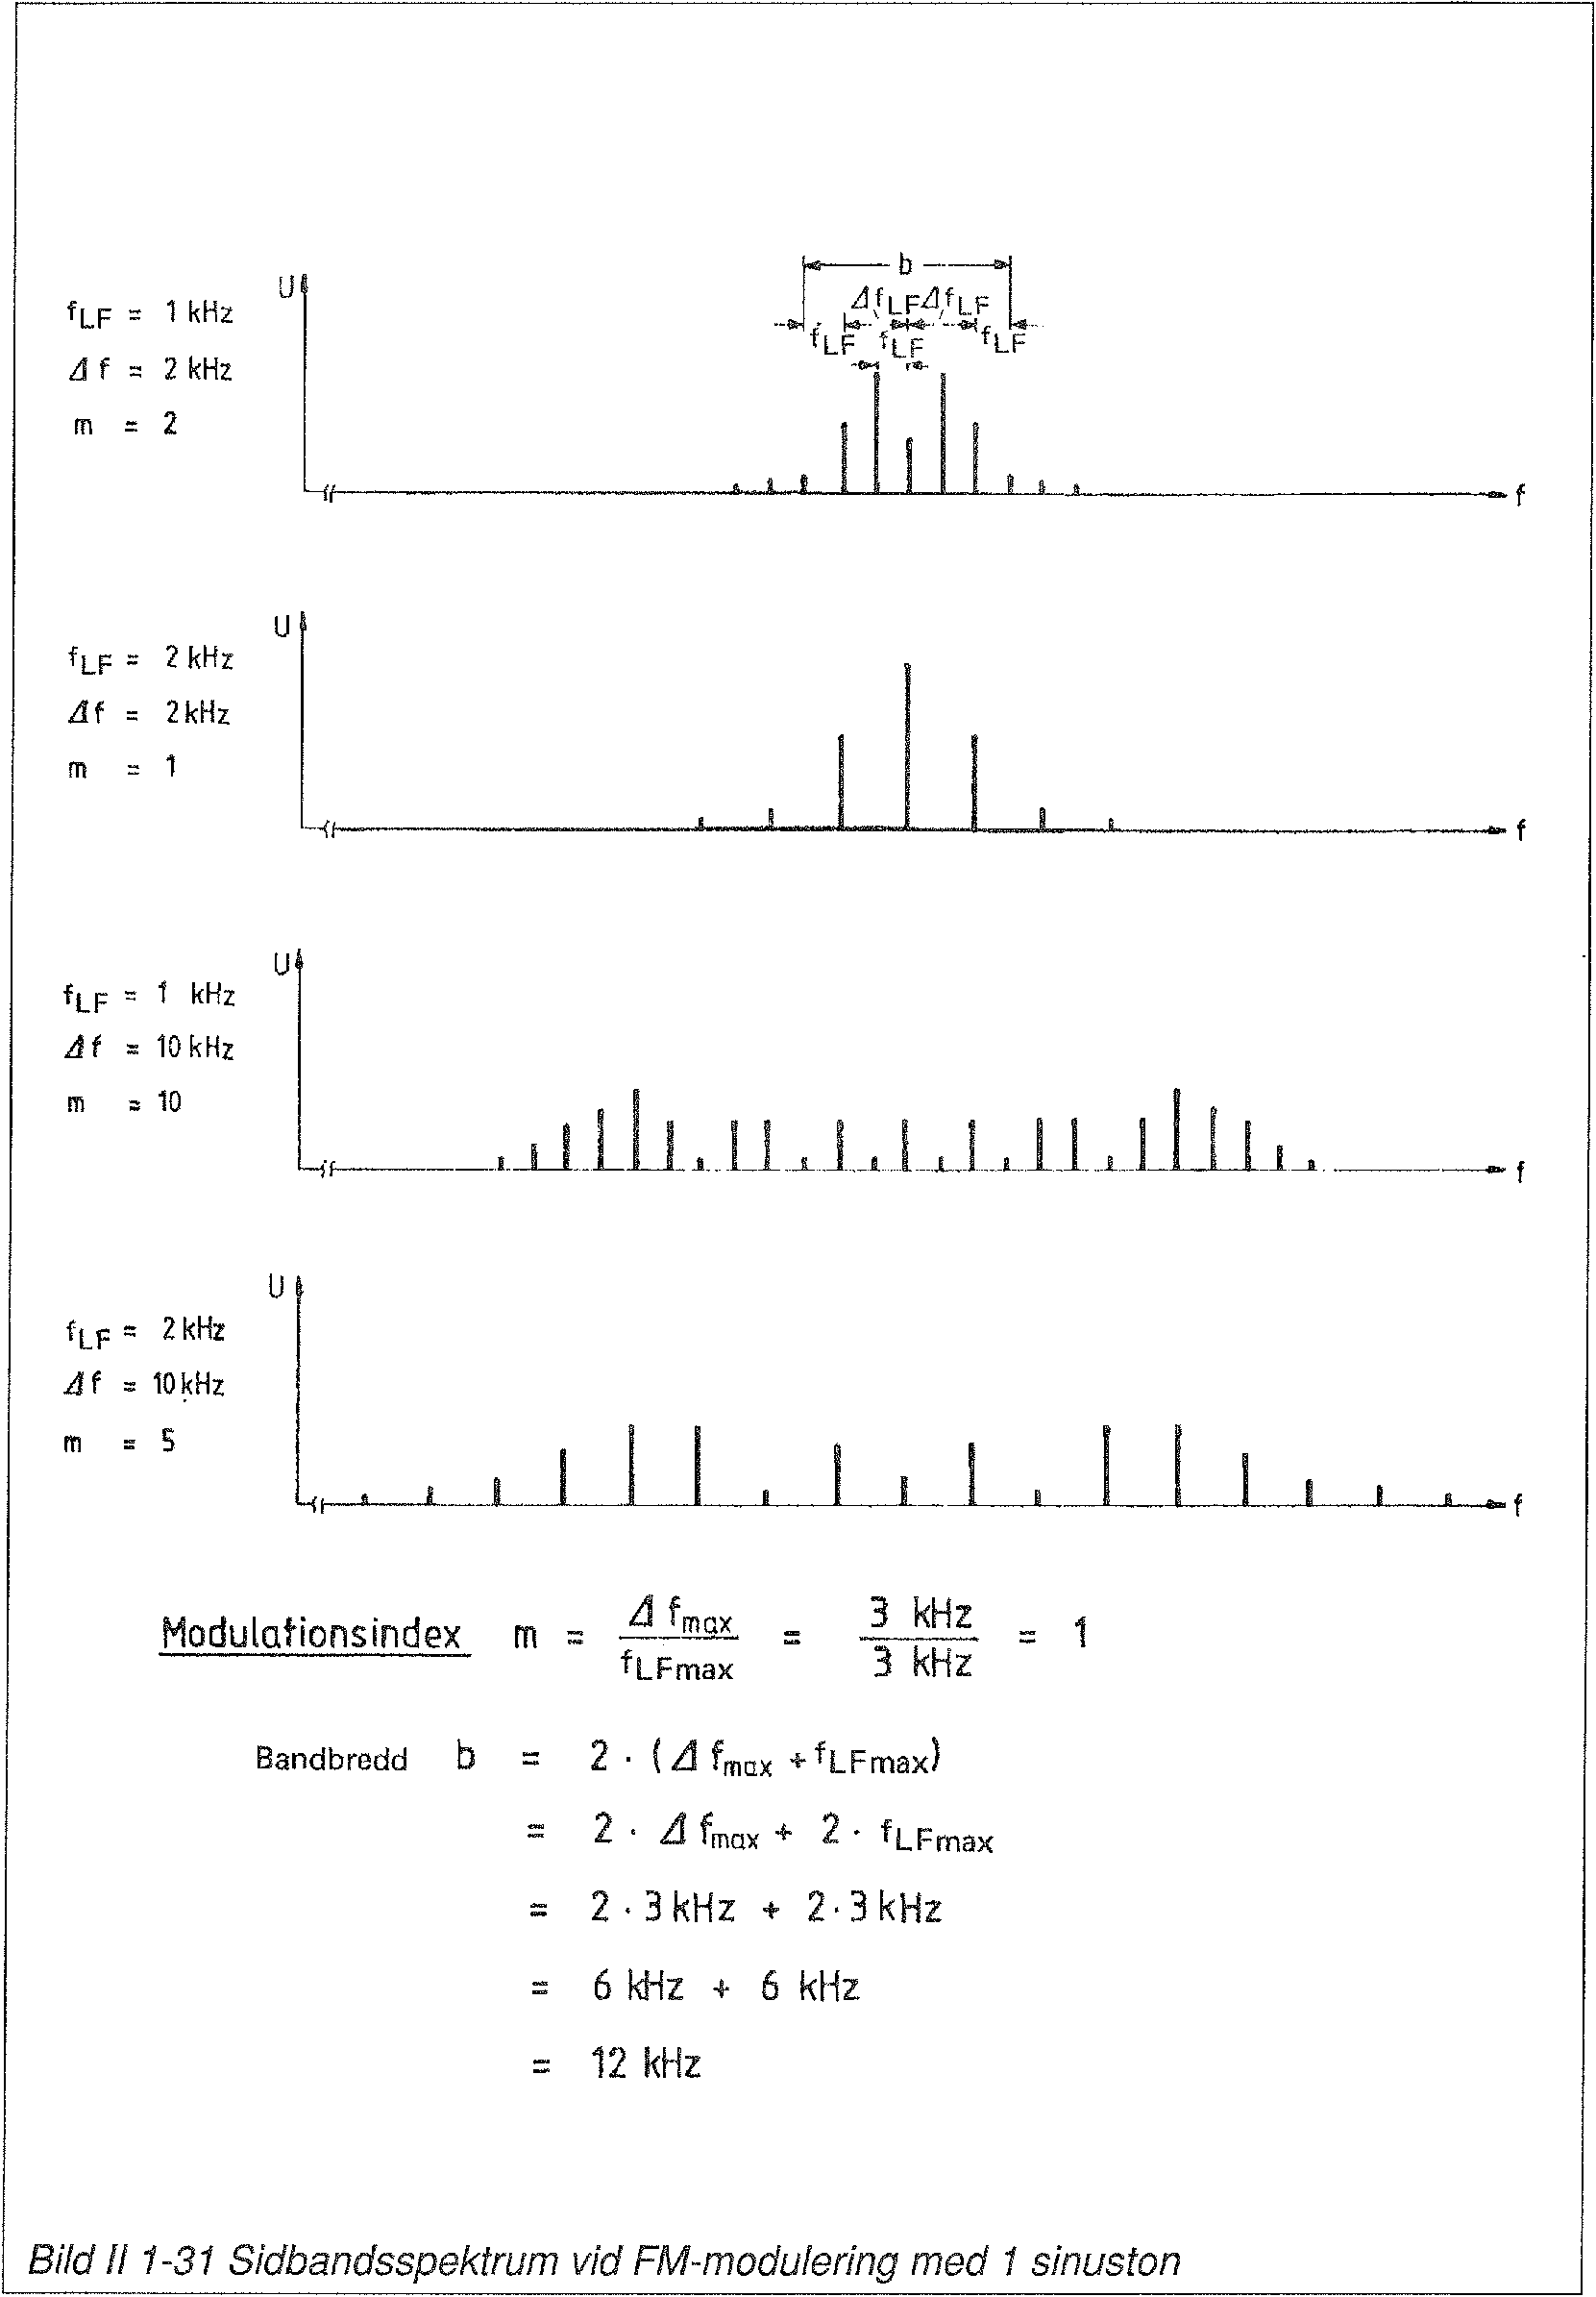
\includegraphics[width=14cm]{images/bild_2_1-31}
\caption{Sidbandsspektrum vid FM-modulering med 1 sinuston}
\label{fig:BildII1-31}
\end{center}
\end{figure*}

Bild \ref{fig:BildII1-31}.

Vid vinkelmodulation uppstår talrika sidefrekvenser, som beror av den
modulerande frekvensen \(f_{LF}\). Amplitudfördelningen mellan sidfrekvenserna
står i förhållande till deviationen, varvid deras amplitud blir mindre desto
längre bort från bärvågen de är.

I praktiken anses en sidfrekvens försumbar när dess amplitud är mindre än 1 \%
av amplituden för omodulerad bärvåg.

För beräkning av bandbredden används begreppet modulationsindex m, vilket är
kvoten av maximal deviation \(\Delta f\) och högsta frekvensen \(f_{LF}\).

\(m = \frac{\Delta f_{max}}{f_{LFmax}}\)

Inom amatörradion är det vanligt att arbeta med \(\Delta f_{max} = 3 kHz\) och
\(f_{LFmax} = 3 kHz\), d.v.s. \(m = 1\).

Vid modulationsindex \(m = 1\), gäller följande
formel för bandbredden \(b\)

\(b = 2 \cdot ( \Delta f_{max} + f_{LFmax}) = 2 \cdot \Delta f_{max}
 + 2 \cdot f_{LFmax}\)

Med ovan nämnda värden blir bandbredden \(b = 2 \cdot (3 kHz + 3 kHz)
 = 12 kHz\)

Bandbredden ökar således både med ökande deviation och ökande modulerande
frekvens. För att inte interferera med trafik på grannkanalerna måste såväl
deviation som frekvensen på den modulerande signalen begränsas. En
deviationsbegränsare begränsar amplituden på denna signal. Ett lågpassfilter
reducerar den distorsion, som uppstår av begränsningen. Vidare undertrycks
modulerande frekvenser högre än 3 kHz, vilket är tillräckligt för överföring
av tal.

\paragraph{Jämförelse}

En VHF-rundradiosändare är tilldelad ett större frekvensutrymme och kan därför
använda mycket större bandbredd

Där är \(\Delta f_{max} = 75 kHz\) och \(f_{LFmax} =15 kHz\), därmed är
\(m = \frac{75}{15} = 5\) och \(b = 2 \cdot (75 + 15) = 180 kHz\).

Som framgår av tabellen på nästa uppslag varierar bärvågens liksom
sidfrekvensernas inbördes amplitud med modulationsindex. Detta skall jämföras
med AM där bärvågens amplitud är konstant och endast sidbandens amplitud
varierar.

Vid vinkelmodulation utsläcks bärvågen \(A_0\) vid modulationsindex 2.404. Den
blir sedan "negativ" vid högre index, vilket betyder att den återkommer, men
att dess fasläge blir omvänt. I vinkelmodulation tas energin i sidbanden från
bärvågen, vilket innebär att den totala effekten förblir densamma oavsett
modulationsindex.

\paragraph{Kännetecken för sändningsslaget F3E (FM)}

Fördelar: F3E-sändaren är enkel till sin uppbyggnad och hög överföringskvalitet
uppnås vid stor bandbredd, störningar från amplitudmodulerade signaler t.ex.
tändgnistor undertrycks i mottagaren.

Nackdelar: En relativt stor bandbredd behövs för överföring av ett basband med
stort frekvensomfång. Sändaren måste avge full effekt, även när modulation inte
sker.

\begin{table*}[h]
\begin{center}
\begin{tabular}{ll|l|l|l|l|l|l|l|l|}
\cline{3-9}
&\multicolumn{1}{l}{}  & \multicolumn{7}{|c|}{Modulationsindex} \\ \cline{3-9}
&\multicolumn{1}{l|}{}  &   1   &   2   &    3   &    4   &    5   &    6   &    7   \\ \hline
\multicolumn{1}{|c|}{\multirow{11}{*}{\rotatebox[origin=c]{90}{Relativ amplitud på}}}&\(A_0\) & 0.765 & 0.224 & -0.260 & -0.397 & -0.178 &  0.151 &  0.300 \\
\multicolumn{1}{|c|}{}&\(A_1\) & 0.440 & 0.577 &  0.334 & -0.066 & -0.328 & -0.277 & -0.005 \\
\multicolumn{1}{|c|}{}&\(A_2\) & 0.115 & 0.353 &  0.486 &  0.364 &  0.047 & -0.243 & -0.301 \\
\multicolumn{1}{|c|}{}&\(A_3\) & 0.020 & 0.129 &  0.309 &  0.430 &  0.365 &  0.115 & -0.168 \\
\multicolumn{1}{|c|}{}&\(A_4\) &       & 0.034 &  0.132 &  0.281 &  0.391 &  0.358 &  0.158 \\
\multicolumn{1}{|c|}{}&\(A_5\) &       & 0.016 &  0.043 &  0.132 &  0.261 &  0.362 &  0.348 \\
\multicolumn{1}{|c|}{}&\(A_6\) & \multicolumn{2}{c|}{} &  0.011 &  0.049 &  0.131 &  0.246 &  0.339 \\
\multicolumn{1}{|c|}{}&\(A_7\) & \multicolumn{3}{c|}{} &  0.015 &  0.053 &  0.130 &  0.234 \\
\multicolumn{1}{|c|}{}&\(A_8\) & \multicolumn{4}{c|}{}           &  0.018 &  0.057 &  0.128 \\
\multicolumn{1}{|c|}{}&\(A_9\) & \multicolumn{4}{c}{} &        &  0.021 &  0.059 \\
\multicolumn{1}{|c|}{}&\(A_{10}\) & \multicolumn{5}{c}{Tomma fält för \(A_n\) under 0.01 (1 \%)} &  &  0.024 \\ \hline
\end{tabular}
\end{center}
\caption{Relativa amplituden på bärvåg \(A_0\) och sidfrekvenser \(A_1\)-\(A_{10}\) vid
modulationsindex 1-7 (Vid omodulerad bärvåg är modulationsindex 0. Då är
bärvågens relativa amplitud 1.0)}
\end{table*}


\subsection{Fasmodulation (även kallat PM)}

Vid fasmodulation varierar bärvågens fasläge i förhållande till ett
referensvärde. Vid PM är frekvensändringen - deviationen - direkt proportionell
till hur snabbt fasläget på den modulerande frekvensen ändras och till den
totala fasändringen. Hastigheten på fasändringen är direkt proportionell till
frekvensen på den modulerande frekvensen och till den momentana amplituden på
den modulerande signalen.

Det betyder att deviationen i PM-system ökar både med den momentana amplituden
och frekvensen på den modulerande signalen. Detta att jämföras med FM-system där
deviationen är proportionell till den momentana amplituden på den modulerande
signalen.

I PM-system uppfattar demodulatorn i mottagaren endast momentana ändringar i
bärvågsfrekvensen. Till skillnad från vid FM, så kan därför ändringar i
likspänningsnivåer överföras endast om en fasreferens används.

Med konstant amplitud på insignalen till modulatorn, så är vid PM
modulationsindex konstant oavsett modulerande frekvens, medan vid FM
modulationsindex varierar med den modulerande frekvensen.

\subsection{Frekvens- och fasmodulation jämförs}

\begin{itemize}
\item Frekvensmodulation (FM) alstras genom att sändarens oscillatorfrekvens
varieras (devieras) i takt med den modulerande signalen (t.ex. tal). Det gör man
genom att variera resonansfrekvensen i den svängningskrets som styr
oscillatorfrekvensen.

\item Fasmodulation (PM) alstras vanligen genom att efter sändarescillatorn
variera den modulerande signalens fasläge i förhållande till en omodulerad
bärvåg - s.k. fasmodulering. Det gör man genom att variera resonansfrekvensen i
en svängningskrets efter oscillatorn- d.v.s. utan att påverka
oscillatorfrekvensen.

\item I båda fallen ändrar man alltså resonansfrekvensen i en svängningskrets i
takt med frekvensen i den modulerande spänningen, men att denna krets har olika
placering i FM-sändare respektive PM-sändare.

\item I sändaren alstras det i båda fallen utfrekvensersom devierarfrån
oscillatorns vilofrekvens. Graden av deviation skiljer emellertid vid FM och PM.
Vid FM är deviationen proportionell mot amplituden på den modulerande
underbärvågen medan deviationen vid PM är proportionell mot produkten av den
modulerande underbärvågens amplitud och frekvens.

\item Den hörbara skillnaden mellan FM och PM är därför en annorlunda
frekvensgång. Vid samtidig användning av PM-sändare och FM-mottagare är det
alltså lämpligt att justera frekvensgången i PM-sändarens modulator, lämpligen
med 6 dB dämpning per oktav ökad frekvens.
\end{itemize}

\subsection{Pulsmodulation}

Pulsmodulation används mest i mikrovågområdet. Pulsmodulerade signaler sänds
vanligen som en serie korta pulser åtskilda av relativt långa pauser utan
modulering.

En typisk sändning kan bestå av pulser med en längd av 1 \(\mu\)s och en
frekvens av 1000 Hz. Toppeffekten på en pulssändning är därför mycket högre än
dess medeleffekt

Före WARC 79 var symbolen för all pulssändning P. Därefter används P endast för
omodulerade pulståg. Annan pulsmodulation har följande symboler

\begin{description}
\item[K] - puls-/amplitudmodulation (PAM)
\item[L] - pulsviddmodulation (PWM)
\item[M] - pulsposition/fasmodulation (PPM)
\item[Q] - vinkelmodulation under pulsen
\item[V] - kombination av dessa eller annat sätt.
\end{description}

\begin{table*}[h]
\begin{center}
\begin{tabular}{|l|l|l|l|l|}
\hline
Sändningsslag & Amplituden på & Tonhöjden på & Bandbredden b      & För stor amplitud \\
              & LF-signa!en   & LF-signalen  & förhåller sig till & på LF-signalen \\
              & påverkar      & påverkar     &                    & medför \\ \hline
A3E (AM) & amplituden i   & sidfrekvenser- & LF-signalens    & övermodulering \\
         & båda sidbanden & nas avstånd    & högsta frekvens & och för stor bandbredd \\
         &                & från bärvågen  & & \\
J3E (SSB)& amplituden på  & sidfrekvenser- & skillnaden mellan & för stor bandbredd,\\
         & utsänt sidband & nas avstånd    & LF-signalens      & överstyrning av\\
         &                & från bärvågen  & högsta och lägsta & förstärkarsteg\\
         &                &                & frekvens          & \\
F3E (FM) & deviationen    & hastigheten på & dubbla summan     & för stor deviation,\\
         &                & bärvågens      & av största devia- & för stor bandbredd\\
         &                & frekvens-      & tion och högsta   & \\
         &                & ändring        & LF-frekvens       & \\ \hline
\end{tabular}
\end{center}
\caption{Jämförelse mellan några. vanliga. sändningsslag inom amatörradio}
\end{table*}
